\documentclass[12pt]{article}

% Font Encoding
\usepackage[T1]{fontenc}

% Page Layout
\usepackage{geometry}
\geometry{a4paper, left=25mm, right=25mm, top=25mm, bottom=25mm}

% Mathematics
\usepackage{amsmath, amssymb, amsthm}

% General Formatting
\usepackage{setspace}
\usepackage{xcolor}
\usepackage{float}
\usepackage{multirow}
\usepackage{graphicx}
\usepackage{hyperref}

% Code Listings
\usepackage{listings}
\lstset{
    language=Python,
    basicstyle=\ttfamily\footnotesize,
    keywordstyle=\color{blue},
    commentstyle=\color{gray},
    stringstyle=\color{red!60!black},
    numbers=left,
    numberstyle=\tiny\color{gray},
    numbersep=8pt,
    frame=single,
    framesep=4pt,
    breaklines=true,
    breakatwhitespace=false,
    showstringspaces=false,
    tabsize=4,
    captionpos=b,
    aboveskip=10pt,
    belowskip=10pt
}

% Theorem environments
\newtheorem{theorem}{Theorem}
\newtheorem{remark}{Remark}

\onehalfspacing

\begin{document}

\begin{center}
{\LARGE \textbf{Annexures A -- I}}\\[12pt]
{\large Understanding Health Insurance Cost Predictions Using\\
Deep Neural Networks, Monte Carlo Simulation and Shapley Values}\\[8pt]
{\normalsize Thabang Bongani Junior Baloyi (2015015486)}
\end{center}

\vspace{10pt}
\tableofcontents
\clearpage

% =============================================================
% Annexure A: Extended Mathematical Details
% =============================================================
\section{Extended Mathematical Details}
\label{annexure:math_details}

% -------------------------------------------------------------
\subsection{Proof of the Universal Approximation Theorem}
\label{annexure:uat_proof}

\begin{theorem}[Cybenko, 1989; Hornik, Stinchcombe and White, 1989]
\label{thm:uat_annexure}
Let $\sigma : \mathbb{R} \to \mathbb{R}$ be a non-constant, bounded, continuous function (the activation function). Let $I_p = [0,1]^p$ denote the $p$-dimensional unit hypercube. For any continuous function $f : I_p \to \mathbb{R}$ and any $\varepsilon > 0$, there exist an integer $N$, real constants $\alpha_i, b_i \in \mathbb{R}$, and vectors $\mathbf{w}_i \in \mathbb{R}^p$ for $i = 1, \ldots, N$, such that the function
\[
  F(\mathbf{x}) = \sum_{i=1}^{N} \alpha_i \, \sigma\!\bigl(\mathbf{w}_i^\top \mathbf{x} + b_i\bigr)
\]
satisfies
\[
  \sup_{\mathbf{x} \in I_p} \bigl| F(\mathbf{x}) - f(\mathbf{x}) \bigr| < \varepsilon.
\]
\end{theorem}

\begin{proof}
The proof proceeds by contradiction and uses the Hahn--Banach theorem from functional analysis. Define the family
\[
  \mathcal{S} = \bigl\{ \sigma(\mathbf{w}^\top \mathbf{x} + b) : \mathbf{w} \in \mathbb{R}^p,\; b \in \mathbb{R} \bigr\}
\]
and let $\mathcal{M}$ denote the closure of $\operatorname{span}(\mathcal{S})$ in $C(I_p)$ with respect to the supremum norm. We wish to show $\mathcal{M} = C(I_p)$.

Suppose, for contradiction, that $\mathcal{M} \neq C(I_p)$. By the Hahn--Banach theorem, there exists a non-zero bounded linear functional $L \in C(I_p)^*$ such that $L(g) = 0$ for all $g \in \mathcal{M}$. By the Riesz representation theorem, there exists a non-zero finite signed regular Borel measure $\mu$ on $I_p$ such that
\[
  L(g) = \int_{I_p} g(\mathbf{x}) \, \mathrm{d}\mu(\mathbf{x})
\]
for all $g \in C(I_p)$. In particular, for all $\mathbf{w} \in \mathbb{R}^p$ and $b \in \mathbb{R}$,
\[
  \int_{I_p} \sigma(\mathbf{w}^\top \mathbf{x} + b) \, \mathrm{d}\mu(\mathbf{x}) = 0.
\]

The key step, due to Cybenko (1989), shows that for discriminatory activation functions (which include all bounded, non-constant, continuous $\sigma$), the condition above forces $\mu = 0$, contradicting the assumption that $L$ is non-zero. The discriminatory property is established by noting that for any half-space $H = \{\mathbf{x} : \mathbf{w}^\top \mathbf{x} + b > 0\}$, the pointwise limit
\[
  \sigma(\lambda \mathbf{w}^\top \mathbf{x} + \lambda b) \to
  \begin{cases}
    1 & \text{if } \mathbf{w}^\top \mathbf{x} + b > 0, \\
    0 & \text{if } \mathbf{w}^\top \mathbf{x} + b < 0,
  \end{cases}
  \quad \text{as } \lambda \to +\infty,
\]
combined with dominated convergence, yields $\mu(H) = 0$ for all open half-spaces $H$. Since open half-spaces generate the Borel $\sigma$-algebra on $I_p$, it follows that $\mu = 0$, a contradiction.
\end{proof}

% -------------------------------------------------------------
\subsection{Derivation of the Adam and NAdam Update Rules}
\label{annexure:adam_nadam}

\paragraph{Adam update rule.}
Let $g_t = \nabla_{\boldsymbol{\theta}} \mathcal{L}(\boldsymbol{\theta}_{t-1})$ denote the gradient of the loss at iteration $t$. The first and second moment estimates are
\begin{align}
  m_t &= \beta_1 \, m_{t-1} + (1 - \beta_1) \, g_t, \label{eq:adam_m} \\
  v_t &= \beta_2 \, v_{t-1} + (1 - \beta_2) \, g_t^2, \label{eq:adam_v}
\end{align}
where $\beta_1, \beta_2 \in [0, 1)$ are the decay rates and the squaring in~\eqref{eq:adam_v} is element-wise. Since $m_0 = v_0 = \mathbf{0}$, these estimates are biased towards zero, especially in early iterations. The bias-corrected estimates are
\begin{align}
  \hat{m}_t &= \frac{m_t}{1 - \beta_1^t}, \label{eq:adam_mhat} \\
  \hat{v}_t &= \frac{v_t}{1 - \beta_2^t}. \label{eq:adam_vhat}
\end{align}
The parameter update is
\begin{equation}
  \boldsymbol{\theta}_t = \boldsymbol{\theta}_{t-1} - \eta \, \frac{\hat{m}_t}{\sqrt{\hat{v}_t} + \epsilon},
  \label{eq:adam_update}
\end{equation}
where $\eta > 0$ is the learning rate and $\epsilon > 0$ (typically $10^{-8}$) prevents division by zero.

\paragraph{NAdam update rule.}
NAdam incorporates Nesterov momentum by replacing the bias-corrected first moment $\hat{m}_t$ with a look-ahead estimate. The modification replaces~\eqref{eq:adam_update} with
\begin{equation}
  \boldsymbol{\theta}_t = \boldsymbol{\theta}_{t-1} - \eta \, \frac{\beta_1 \hat{m}_t + \frac{(1-\beta_1)}{1-\beta_1^t} g_t}{\sqrt{\hat{v}_t} + \epsilon}.
  \label{eq:nadam_update}
\end{equation}
% -------------------------------------------------------------
\subsection{Shapley Value Axiom Verification}
\label{annexure:shapley_axioms}

\paragraph{Axiom 1: Efficiency.}
\[
  \sum_{j=1}^{p} \phi_j(v) = v(N) - v(\emptyset).
\]

\paragraph{Axiom 2: Symmetry.}
If two players $j$ and $k$ contribute equally to every coalition, i.e.\ $v(S \cup \{j\}) = v(S \cup \{k\})$ for all $S \subseteq N \setminus \{j,k\}$, then $\phi_j(v) = \phi_k(v)$.

\paragraph{Axiom 3: Dummy player.}
If player $j$ adds nothing to any coalition, i.e.\ $v(S \cup \{j\}) = v(S)$ for all $S \subseteq N \setminus \{j\}$, then $\phi_j(v) = 0$.

\paragraph{Axiom 4: Additivity (linearity).}
For two games $v$ and $w$, the Shapley value of the combined game $v + w$ is $\phi_j(v + w) = \phi_j(v) + \phi_j(w)$ for all $j$.

\begin{theorem}[Shapley, 1953]
\label{thm:shapley_uniqueness}
There exists a unique function $\phi : \mathcal{G}^N \to \mathbb{R}^p$ satisfying Axioms 1--4, and it is given by
\[
  \phi_j(v) = \sum_{S \subseteq N \setminus \{j\}} \frac{|S|!\;(p - |S| - 1)!}{p!} \bigl[ v(S \cup \{j\}) - v(S) \bigr].
\]
\end{theorem}

\begin{proof}
\emph{Existence} is verified by direct calculation: substituting the formula into each axiom confirms that all four hold.

\emph{Uniqueness} proceeds by induction on the number of players. For $p = 1$, efficiency forces $\phi_1(v) = v(\{1\}) - v(\emptyset)$, which is unique. For the inductive step, any game $v$ can be decomposed as a linear combination of unanimity games $u_T$ (where $u_T(S) = 1$ if $T \subseteq S$ and $u_T(S) = 0$ otherwise). By additivity, it suffices to determine $\phi_j(u_T)$. By the dummy axiom, $\phi_j(u_T) = 0$ for $j \notin T$. By symmetry, $\phi_j(u_T) = \phi_k(u_T)$ for all $j, k \in T$. By efficiency, $\sum_{j \in T} \phi_j(u_T) = 1$. Hence $\phi_j(u_T) = 1/|T|$ for $j \in T$, which uniquely determines $\phi$ for all unanimity games, and by linearity, for all games.
\end{proof}

% -------------------------------------------------------------
\subsection{Gamma GLM Log-Link Score Equations}
\label{annexure:glm_score}

The expected response is $\mu_i = \exp(\mathbf{x}_i^\top \boldsymbol{\beta})$. The Gamma density with shape parameter $\alpha$ and mean $\mu$ is
\[
  f(y; \alpha, \mu) = \frac{1}{\Gamma(\alpha)} \left( \frac{\alpha}{\mu} \right)^\alpha y^{\alpha - 1} \exp\!\left( -\frac{\alpha y}{\mu} \right), \quad y > 0.
\]

The log-likelihood for observation $i$ (up to a constant not depending on $\boldsymbol{\beta}$) is
\[
  \ell_i(\boldsymbol{\beta}) = -\alpha \log \mu_i - \frac{\alpha y_i}{\mu_i} = -\alpha \, \mathbf{x}_i^\top \boldsymbol{\beta} - \alpha \, y_i \exp(-\mathbf{x}_i^\top \boldsymbol{\beta}).
\]

The score equation with respect to the $k$-th coefficient is obtained by differentiating $\ell = \sum_{i=1}^{n} \ell_i$:
\begin{equation}
  \frac{\partial \ell}{\partial \beta_k} = \alpha \sum_{i=1}^{n} \left( \frac{y_i}{\mu_i} - 1 \right) x_{ik} = 0, \quad k = 0, 1, \ldots, p.
  \label{eq:glm_score}
\end{equation}

Since $\alpha > 0$ cancels, the maximum-likelihood estimates $\hat{\boldsymbol{\beta}}$ do not depend on the shape parameter. The Fisher information matrix entry is
\[
  \mathcal{I}_{kl} = \alpha \sum_{i=1}^{n} \mu_i^{-1} \, x_{ik} \, x_{il},
\]
and the asymptotic covariance of $\hat{\boldsymbol{\beta}}$ is $\mathcal{I}^{-1}$.


\clearpage
% =============================================================
% Annexure B: Data Preprocessing and Encoding
% =============================================================
\section{Data Preprocessing and Encoding}
\label{annexure:preprocessing}

The raw dataset contains 1\,000\,000 rows and 12 columns. The preprocessing procedure consists of four stages: data auditing, reference-category encoding, partitioning and input standardisation.

% -------------------------------------------------------------
\subsection{Data Audit}
\label{annexure:data_loading}

The data audit confirmed no missing values in numeric columns, no exact duplicate rows, and that all categorical levels matched the expected domain. Missing values in \texttt{medical\_history} and \texttt{family\_medical\_history} were coded as \texttt{None} and treated as a valid reference level.

% -------------------------------------------------------------
\subsection{Reference-Category Encoding}
\label{annexure:encoding}

Each categorical variable was encoded using reference-category (dummy) coding, producing 22 numeric features from the original 11 input variables. Table~\ref{tab:reference_categories} lists the reference category for each variable.

\begin{table}[htbp]
\centering
\caption{Reference categories used in dummy encoding.}
\label{tab:reference_categories}
\begin{tabular}{ll}
\toprule
\textbf{Variable} & \textbf{Reference Category} \\
\midrule
region                    & northeast \\
medical\_history          & None \\
family\_medical\_history  & None \\
exercise\_frequency       & Rarely \\
occupation                & Unemployed \\
coverage\_level           & Basic \\
\bottomrule
\end{tabular}
\end{table}

Binary variables (gender, smoker) were coded as single indicator columns. Numeric variables (age, bmi, children) were passed through without transformation.

% -------------------------------------------------------------
\subsection{Data Partitioning}
\label{annexure:split}

The encoded dataset was split into training (60\%), validation (20\%) and test (20\%) partitions using random sampling with \texttt{random\_state=42}.

% -------------------------------------------------------------
\subsection{Input Standardisation}
\label{annexure:standardisation}

All 22 input features were standardised to zero mean and unit variance using parameters computed from the training partition only. The response variable (charges) was similarly standardised. Binary dummy columns with zero variance in the training set were protected by setting their standard deviation to 1.0 before division.

\begin{algorithm}[htbp]
\caption{Data preprocessing and standardisation.}
\label{alg:preprocessing}
\begin{algorithmic}[1]
\Require Raw dataset $\mathcal{D}$ with $n$ rows and 12 columns
\Ensure Standardised feature matrices $\mathbf{X}_{\mathrm{train}}, \mathbf{X}_{\mathrm{val}}, \mathbf{X}_{\mathrm{test}}$ and response vectors $\mathbf{y}_{\mathrm{train}}, \mathbf{y}_{\mathrm{val}}, \mathbf{y}_{\mathrm{test}}$
\State Fill missing values in categorical columns with reference level
\State Apply reference-category encoding to obtain $n \times 22$ feature matrix
\State Split: $\mathcal{D}_{\mathrm{train}}$ (60\%), $\mathcal{D}_{\mathrm{val}}$ (20\%), $\mathcal{D}_{\mathrm{test}}$ (20\%) with seed 42
\State Compute $\boldsymbol{\mu}_X, \boldsymbol{\sigma}_X$ from $\mathcal{D}_{\mathrm{train}}$ features only
\State Compute $\mu_y, \sigma_y$ from $\mathcal{D}_{\mathrm{train}}$ response only
\For{each partition $\mathcal{P} \in \{\mathrm{train}, \mathrm{val}, \mathrm{test}\}$}
    \State $\mathbf{X}_{\mathcal{P}} \gets (\mathbf{X}_{\mathcal{P}}^{\mathrm{raw}} - \boldsymbol{\mu}_X) \,/\, \boldsymbol{\sigma}_X$
    \State $\mathbf{y}_{\mathcal{P}} \gets (\mathbf{y}_{\mathcal{P}}^{\mathrm{raw}} - \mu_y) \,/\, \sigma_y$
\EndFor
\end{algorithmic}
\end{algorithm}

\subsection{Response De-normalisation}
\label{annexure:denormalise}

Predictions on the normalised scale are converted back to the original Rand scale via $\hat{y} = \hat{y}_{\mathrm{norm}} \cdot \sigma_y + \mu_y$, where $\mu_y$ and $\sigma_y$ are the training-set response mean and standard deviation respectively.


\clearpage
% =============================================================
% Annexure C: DNN Architecture and Training Procedure
% =============================================================
\section{DNN Architecture and Training Procedure}
\label{annexure:dnn_training}

The FunnelDNN model uses a feed-forward architecture with monotonically decreasing hidden layer widths: $22 \to 256 \to 128 \to 64 \to 32 \to 16 \to 1$. All layers are bias-free, and the CELU activation function is applied after each hidden layer. The output layer is linear with no activation.

% -------------------------------------------------------------
\subsection{Training Procedure}
\label{annexure:train_model}

Training minimises the mean squared error loss on normalised data using the NAdam optimiser. Validation-based early stopping monitors the dot-product $R^2$ on the validation set every 5 epochs, with a patience of 10 checks.

\begin{algorithm}[htbp]
\caption{FunnelDNN training with early stopping.}
\label{alg:dnn_training}
\begin{algorithmic}[1]
\Require Standardised data $(\mathbf{X}_{\mathrm{train}}, \mathbf{y}_{\mathrm{train}}, \mathbf{X}_{\mathrm{val}}, \mathbf{y}_{\mathrm{val}})$, learning rate $\eta$, batch size $B$, patience $P$, validation interval $V$
\Ensure Trained model state $\boldsymbol{\theta}^*$
\State Initialise FunnelDNN with seed 42
\State $\boldsymbol{\theta}^* \gets \boldsymbol{\theta}_0$, \; $R^{2*} \gets -\infty$, \; $c \gets 0$
\For{$t = 1, 2, \ldots, T_{\max}$}
    \For{each mini-batch $(\mathbf{X}_b, \mathbf{y}_b)$ of size $B$}
        \State Compute $\mathcal{L} = \mathrm{MSE}\bigl(f_{\boldsymbol{\theta}}(\mathbf{X}_b),\, \mathbf{y}_b\bigr)$
        \State Update $\boldsymbol{\theta}$ via NAdam with learning rate $\eta$
    \EndFor
    \If{$t \bmod V = 0$}
        \State Compute $R^2_{\mathrm{val}} = r^2_{\mathrm{dot}}\bigl(\mathbf{y}_{\mathrm{val}},\, f_{\boldsymbol{\theta}}(\mathbf{X}_{\mathrm{val}})\bigr)$
        \If{$R^2_{\mathrm{val}} > R^{2*}$}
            \State $R^{2*} \gets R^2_{\mathrm{val}}$, \; $\boldsymbol{\theta}^* \gets \boldsymbol{\theta}$, \; $c \gets 0$
        \Else
            \State $c \gets c + 1$
        \EndIf
        \If{$c \geq P$}
            \State \textbf{break} \Comment{Early stopping triggered}
        \EndIf
    \EndIf
\EndFor
\State \Return $\boldsymbol{\theta}^*$
\end{algorithmic}
\end{algorithm}

% -------------------------------------------------------------
\subsection{Evaluation Metrics}
\label{annexure:eval_helpers}

Three metrics are computed on the original Rand scale after de-normalisation:
\begin{itemize}
    \item $R^2 = 1 - \mathrm{SS}_{\mathrm{res}} / \mathrm{SS}_{\mathrm{tot}}$, where $\mathrm{SS}_{\mathrm{res}} = \sum_i (y_i - \hat{y}_i)^2$ and $\mathrm{SS}_{\mathrm{tot}} = \sum_i (y_i - \bar{y})^2$.
    \item $\mathrm{RMSE} = \sqrt{n^{-1} \sum_i (y_i - \hat{y}_i)^2}$.
    \item $\mathrm{MAE} = n^{-1} \sum_i |y_i - \hat{y}_i|$.
\end{itemize}

During training, the dot-product $R^2$ (squared correlation between predicted and observed values) is used on normalised data for computational speed.

% -------------------------------------------------------------
\subsection{Checkpoint Contents}
\label{annexure:final_model}

The final trained model is saved as \texttt{chapter3\_final\_model.pth}, a PyTorch checkpoint containing:
\begin{itemize}
    \item Model weight tensors (state dictionary).
    \item Architecture specification (layer widths, activation, bias setting).
    \item Selected hyperparameters (learning rate, batch size, optimiser, momentum).
    \item Standardisation parameters ($\boldsymbol{\mu}_X$, $\boldsymbol{\sigma}_X$, $\mu_y$, $\sigma_y$).
    \item Feature names and evaluation metrics.
\end{itemize}


\clearpage
% =============================================================
% Annexure D: Code for Monte Carlo Simulation
% =============================================================
\section{Code for Monte Carlo Simulation}
\label{annexure:mc_simulation}

% -------------------------------------------------------------
\subsection{Marginal Distribution Estimation}
\label{annexure:mc_marginals}

\begin{lstlisting}[caption={Marginal distribution estimation.}]
import numpy as np
import pandas as pd

df_raw = pd.read_csv('insurance_dataset.csv')
df_raw['medical_history'] = (
    df_raw['medical_history'].fillna('None'))
df_raw['family_medical_history'] = (
    df_raw['family_medical_history'].fillna('None'))

p_male = (df_raw['gender'] == 'male').mean()
p_smoker = (df_raw['smoker'] == 'yes').mean()

region_levels = ['northeast', 'northwest',
                 'southeast', 'southwest']
region_probs = np.array(
    [(df_raw['region'] == r).mean()
     for r in region_levels])

med_hist_levels = ['None', 'Heart disease',
                   'High blood pressure', 'Diabetes']
med_hist_probs = np.array(
    [(df_raw['medical_history'] == m).mean()
     for m in med_hist_levels])

fam_hist_levels = ['None', 'Heart disease',
                   'High blood pressure', 'Diabetes']
fam_hist_probs = np.array(
    [(df_raw['family_medical_history'] == f).mean()
     for f in fam_hist_levels])

exercise_levels = ['Rarely', 'Occasionally',
                   'Frequently', 'Never']
exercise_probs = np.array(
    [(df_raw['exercise_frequency'] == e).mean()
     for e in exercise_levels])

occ_levels = ['Unemployed', 'Student',
              'Blue collar', 'White collar']
occ_probs = np.array(
    [(df_raw['occupation'] == o).mean()
     for o in occ_levels])

cov_levels = ['Basic', 'Standard', 'Premium']
cov_probs = np.array(
    [(df_raw['coverage_level'] == c).mean()
     for c in cov_levels])
\end{lstlisting}

% -------------------------------------------------------------
\subsection{Profile Generation Function}
\label{annexure:mc_generate}

\begin{lstlisting}[caption={\texttt{generate\_mc\_profiles}: generate $B$ synthetic policyholder profiles from fitted marginals.}]
B = 10_000  # Number of MC samples

def generate_mc_profiles(n, rng):
    """Generate n raw MC profiles from fitted marginals.

    Marginal distributions:
        age:      DiscreteUniform(18, 65)
        bmi:      ContinuousUniform(18, 50)
        children: DiscreteUniform(0, 5)
        Categorical variables: Multinomial with
                               estimated proportions
    """
    age = rng.integers(18, 66, size=n)
    bmi = rng.uniform(18.0, 50.0, size=n)
    children = rng.integers(0, 6, size=n)
    gender = rng.choice(['male', 'female'],
                        size=n, p=[p_male, 1-p_male])
    smoker = rng.choice(['yes', 'no'],
                        size=n, p=[p_smoker, 1-p_smoker])
    region = rng.choice(region_levels,
                        size=n, p=region_probs)
    medical_history = rng.choice(
        med_hist_levels, size=n, p=med_hist_probs)
    family_medical_history = rng.choice(
        fam_hist_levels, size=n, p=fam_hist_probs)
    exercise_frequency = rng.choice(
        exercise_levels, size=n, p=exercise_probs)
    occupation = rng.choice(
        occ_levels, size=n, p=occ_probs)
    coverage_level = rng.choice(
        cov_levels, size=n, p=cov_probs)

    return pd.DataFrame({
        'age': age, 'gender': gender,
        'bmi': bmi, 'children': children,
        'smoker': smoker, 'region': region,
        'medical_history': medical_history,
        'family_medical_history':
            family_medical_history,
        'exercise_frequency': exercise_frequency,
        'occupation': occupation,
        'coverage_level': coverage_level
    })
\end{lstlisting}

% -------------------------------------------------------------
\subsection{Profile Encoding Function}
\label{annexure:mc_encode}

\begin{lstlisting}[caption={\texttt{encode\_profiles}: reference-category encoding for MC samples.}]
def encode_profiles(df_mc):
    """Apply reference-category encoding to match
    the 22 model features.

    Returns np.ndarray of shape (n, 22).
    """
    n = len(df_mc)
    X = np.zeros((n, 22), dtype=np.float32)

    X[:, 0] = df_mc['age'].values
    X[:, 1] = (df_mc['gender'] == 'male'
               ).astype(np.float32).values
    X[:, 2] = df_mc['bmi'].values
    X[:, 3] = df_mc['children'].values
    X[:, 4] = (df_mc['smoker'] == 'yes'
               ).astype(np.float32).values

    # region dummies (ref = northeast)
    X[:, 5] = (df_mc['region'] == 'southwest'
               ).astype(np.float32).values
    X[:, 6] = (df_mc['region'] == 'northwest'
               ).astype(np.float32).values
    X[:, 7] = (df_mc['region'] == 'southeast'
               ).astype(np.float32).values

    # medical_history (ref = None)
    X[:, 8] = (df_mc['medical_history']
               == 'Heart disease'
               ).astype(np.float32).values
    X[:, 9] = (df_mc['medical_history']
               == 'High blood pressure'
               ).astype(np.float32).values
    X[:,10] = (df_mc['medical_history']
               == 'Diabetes'
               ).astype(np.float32).values

    # family_medical_history (ref = None)
    X[:,11] = (df_mc['family_medical_history']
               == 'Heart disease'
               ).astype(np.float32).values
    X[:,12] = (df_mc['family_medical_history']
               == 'High blood pressure'
               ).astype(np.float32).values
    X[:,13] = (df_mc['family_medical_history']
               == 'Diabetes'
               ).astype(np.float32).values

    # exercise_frequency (ref = Rarely)
    X[:,14] = (df_mc['exercise_frequency']
               == 'Occasionally'
               ).astype(np.float32).values
    X[:,15] = (df_mc['exercise_frequency']
               == 'Frequently'
               ).astype(np.float32).values
    X[:,16] = (df_mc['exercise_frequency']
               == 'Never'
               ).astype(np.float32).values

    # occupation (ref = Unemployed)
    X[:,17] = (df_mc['occupation'] == 'Student'
               ).astype(np.float32).values
    X[:,18] = (df_mc['occupation'] == 'Blue collar'
               ).astype(np.float32).values
    X[:,19] = (df_mc['occupation'] == 'White collar'
               ).astype(np.float32).values

    # coverage_level (ref = Basic)
    X[:,20] = (df_mc['coverage_level'] == 'Standard'
               ).astype(np.float32).values
    X[:,21] = (df_mc['coverage_level'] == 'Premium'
               ).astype(np.float32).values

    return X
\end{lstlisting}

% -------------------------------------------------------------
\subsection{DNN Scoring Helper}
\label{annexure:mc_score}

\begin{lstlisting}[caption={\texttt{score\_dnn}: standardise, forward-pass, de-normalise.}]
import torch

def score_dnn(X_encoded_raw,
              standardise=True, denormalise=True):
    """Score profiles through the trained DNN.

    Parameters
    ----------
    X_encoded_raw : np.ndarray, shape (n, 22)
    standardise : bool
        Apply (X - X_mean) / X_std before scoring.
    denormalise : bool
        Convert output to original Rand scale.

    Returns
    -------
    np.ndarray, shape (n,)
    """
    X = X_encoded_raw.astype(np.float32)
    if standardise:
        X = (X - X_mean) / X_std
    X_t = torch.tensor(
        X, dtype=torch.float32).to(DEVICE)
    with torch.no_grad():
        preds = model(X_t).cpu().numpy().flatten()
    if denormalise:
        preds = preds * y_std + y_mean
    return preds
\end{lstlisting}

% -------------------------------------------------------------
\subsection{MC Convergence Diagnostics}
\label{annexure:mc_convergence}

\begin{lstlisting}[caption={MC convergence diagnostics.}]
from scipy import stats

pilot_sizes = [1000, 2500, 5000, 10000, 20000]

rng_pilot = np.random.default_rng(SEED)
df_pilot = generate_mc_profiles(
    max(pilot_sizes), rng_pilot)
X_pilot_enc = encode_profiles(df_pilot)
y_pilot = score_dnn(X_pilot_enc)

convergence_stats = []
for B_pilot in pilot_sizes:
    y_sub = y_pilot[:B_pilot]
    row = {
        'B': B_pilot,
        'Mean': y_sub.mean(),
        'SD': y_sub.std(),
        'P50': np.percentile(y_sub, 50),
        'P90': np.percentile(y_sub, 90),
        'P95': np.percentile(y_sub, 95),
        'P99': np.percentile(y_sub, 99),
        'MCSE': y_sub.std() / np.sqrt(B_pilot)
    }
    convergence_stats.append(row)
\end{lstlisting}

% -------------------------------------------------------------
\subsection{Residual-Augmented MC Sensitivity}
\label{annexure:mc_residual}

\begin{lstlisting}[caption={Residual-augmented MC sensitivity.}]
# Compute training residuals
y_train_pred = score_dnn(X_train_raw)
residuals_train = y_train_raw - y_train_pred

# Centre the residuals
residuals_centred = (
    residuals_train - residuals_train.mean())
sigma_e = residuals_centred.std()

# Augmented predictions: Y_res = Y_hat + epsilon
rng_res = np.random.default_rng(SEED + 1)
eps_sample = rng_res.choice(
    residuals_centred, size=B, replace=True)
y_mc_augmented = y_mc + eps_sample

# Fixed perturbation bands
y_mc_upper = y_mc + 0.5 * sigma_e
y_mc_lower = y_mc - 0.5 * sigma_e
\end{lstlisting}


\clearpage
% =============================================================
% Annexure E: Code for GLM Benchmark
% =============================================================
\section{Code for GLM Benchmark}
\label{annexure:glm_benchmark}

% -------------------------------------------------------------
\subsection{GLM Fitting via \texttt{statsmodels}}
\label{annexure:glm_fit}

\begin{lstlisting}[caption={GLM (Gamma, log-link) fitting.}]
import statsmodels.api as sm
import numpy as np

# Add intercept column
X_glm_train = sm.add_constant(X_train_raw)
X_glm_val   = sm.add_constant(X_val_raw)
X_glm_test  = sm.add_constant(X_test_raw)

# Fit GLM with Gamma family and log link
glm_model = sm.GLM(
    y_train_raw,
    X_glm_train,
    family=sm.families.Gamma(
        sm.families.links.Log())
).fit()

# Predictions on all three partitions
glm_pred_train = glm_model.predict(X_glm_train)
glm_pred_val   = glm_model.predict(X_glm_val)
glm_pred_test  = glm_model.predict(X_glm_test)
\end{lstlisting}

% -------------------------------------------------------------
\subsection{Coefficient Table Extraction}
\label{annexure:glm_coefs}

\begin{lstlisting}[caption={GLM coefficient table extraction.}]
import pandas as pd

glm_coef = pd.DataFrame({
    'Feature': ['const'] + FEATURES,
    'Coefficient': glm_model.params,
    'exp(Coef)': np.exp(glm_model.params),
    'Std Error': glm_model.bse,
    'z-value': glm_model.tvalues,
    'p-value': glm_model.pvalues
})
glm_coef['Significant (p<0.05)'] = (
    glm_coef['p-value'] < 0.05)

n_sig = glm_coef['Significant (p<0.05)'].sum()
print(f'{n_sig} of {len(glm_coef)} coefficients '
      f'are significant (p < 0.05).')
\end{lstlisting}

% -------------------------------------------------------------
\subsection{Comparison Metrics Computation}
\label{annexure:glm_metrics}

\begin{lstlisting}[caption={\texttt{compute\_metrics}: $R^2$, RMSE and MAE on the original Rand scale.}]
def compute_metrics(y_true, y_pred):
    """Compute R2, RMSE and MAE."""
    ss_res = np.sum((y_true - y_pred) ** 2)
    ss_tot = np.sum((y_true - y_true.mean()) ** 2)
    r2 = 1 - ss_res / ss_tot if ss_tot > 0 else 0.0
    rmse = np.sqrt(np.mean((y_true - y_pred) ** 2))
    mae = np.mean(np.abs(y_true - y_pred))
    return {'R2': float(r2),
            'RMSE': float(rmse),
            'MAE': float(mae)}
\end{lstlisting}

% -------------------------------------------------------------
\subsection{GLM vs DNN Comparison Table}
\label{annexure:glm_vs_dnn}

\begin{lstlisting}[caption={GLM vs DNN comparison table generation.}]
results = {}

# GLM metrics
results['GLM (Gamma, log-link)'] = {
    'Train': compute_metrics(
        y_train_raw, glm_pred_train),
    'Validation': compute_metrics(
        y_val_raw, glm_pred_val),
    'Test': compute_metrics(
        y_test_raw, glm_pred_test)
}

# DNN metrics (from checkpoint evaluation)
results['DNN (Funnel)'] = {
    'Train': compute_metrics(
        y_train_raw, dnn_pred_train),
    'Validation': compute_metrics(
        y_val_raw, dnn_pred_val),
    'Test': compute_metrics(
        y_test_raw, dnn_pred_test)
}

# Print comparison
model_order = ['GLM (Gamma, log-link)',
               'DNN (Funnel)']
print(f'{"Model":<25} {"Set":<12} '
      f'{"R2":>10} {"RMSE":>12} {"MAE":>12}')
for model_name in model_order:
    for set_name in ['Train', 'Validation', 'Test']:
        m = results[model_name][set_name]
        print(f'{model_name:<25} {set_name:<12} '
              f'{m["R2"]:>10.6f} '
              f'{m["RMSE"]:>12.2f} '
              f'{m["MAE"]:>12.2f}')

# Save to CSV
rows = []
for model_name in model_order:
    for set_name in ['Train', 'Validation', 'Test']:
        m = results[model_name][set_name]
        rows.append({
            'Model': model_name,
            'Set': set_name,
            'R2': round(m['R2'], 6),
            'RMSE': round(m['RMSE'], 2),
            'MAE': round(m['MAE'], 2)
        })

df_comparison = pd.DataFrame(rows)
df_comparison.to_csv(
    'glm_vs_dnn_comparison.csv', index=False)
\end{lstlisting}

\begin{figure}[H]
    \centering
    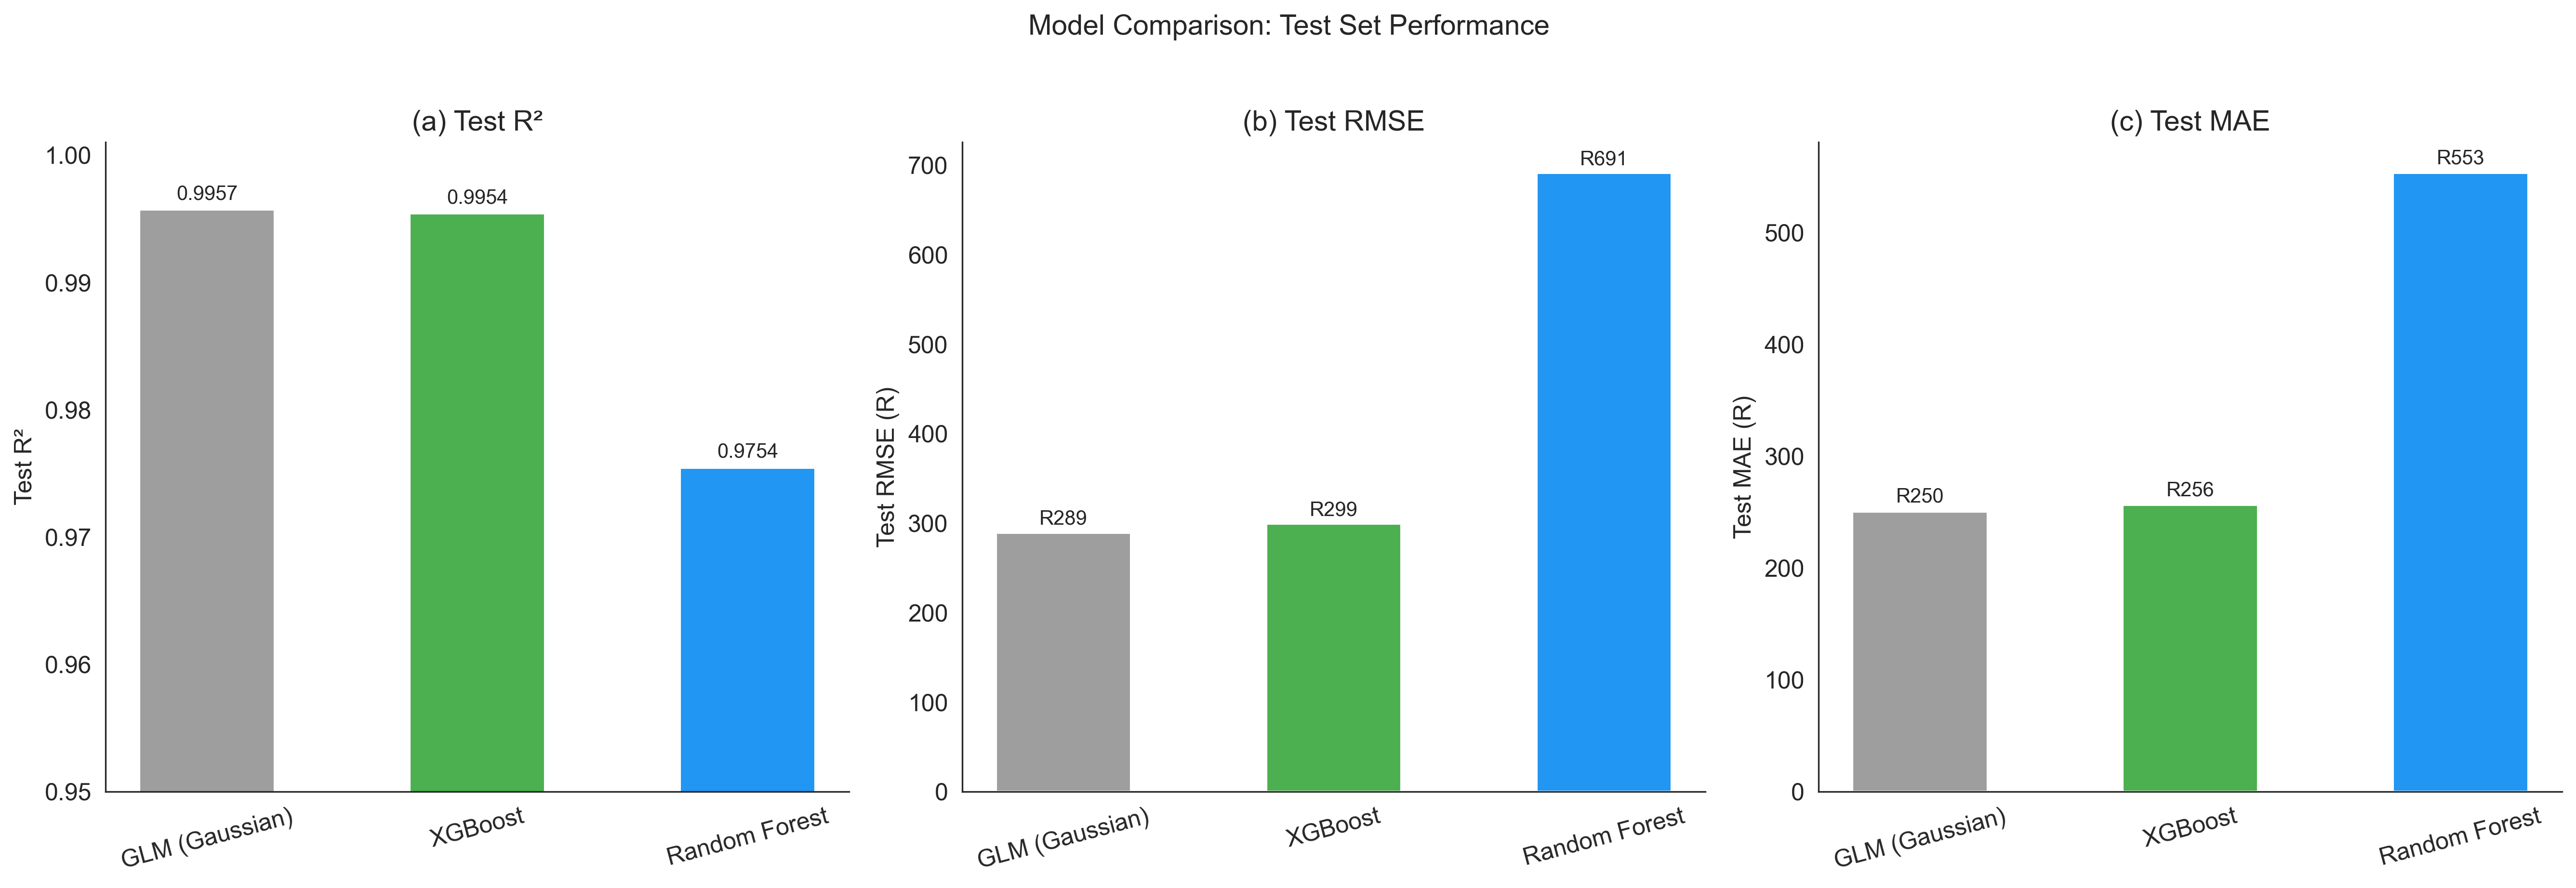
\includegraphics[width=0.9\textwidth]{Thesis/Chapter 4/Figures/fig_full_model_comparison.png}
    \caption{Full model comparison.}
    \label{fig:annexure_full_model_comparison}
\end{figure}


\clearpage
% =============================================================
% Annexure F: Code for Shapley-Value Computation
% =============================================================
\section{Code for Shapley-Value Computation}
\label{annexure:shapley}

% -------------------------------------------------------------
\subsection{SHAP GradientExplainer Setup}
\label{annexure:shap_setup}

\begin{lstlisting}[caption={SHAP GradientExplainer initialisation.}]
import copy
import shap
import torch
import numpy as np

# CPU copy for SHAP (faster than MPS for
# GradientExplainer)
model_cpu = copy.deepcopy(model).cpu()
model_cpu.eval()

# Background: 200 randomly sampled
# standardised training rows
rng = np.random.default_rng(SEED)
bg_idx = rng.choice(len(X_train_std),
                     200, replace=False)
X_bg = torch.tensor(X_train_std[bg_idx],
                    dtype=torch.float32)

# Foreground: all MC profiles (standardised)
X_mc_std = ((X_mc_encoded - X_mean) / X_std
            ).astype(np.float32)
X_fg = torch.tensor(X_mc_std,
                    dtype=torch.float32)

explainer = shap.GradientExplainer(
    model_cpu, X_bg)
\end{lstlisting}

% -------------------------------------------------------------
\subsection{Batch SHAP Computation}
\label{annexure:shap_batch}

\begin{lstlisting}[caption={Batch SHAP computation.}]
BATCH_SHAP = 2000
shap_values_list = []
n_batches = (B + BATCH_SHAP - 1) // BATCH_SHAP

for i in range(n_batches):
    start = i * BATCH_SHAP
    end = min((i + 1) * BATCH_SHAP, B)
    sv = explainer.shap_values(X_fg[start:end])

    if isinstance(sv, list):
        sv = sv[0]
    if isinstance(sv, torch.Tensor):
        sv = sv.cpu().numpy()
    # GradientExplainer returns shape (n, 22, 1)
    # for single-output models
    if sv.ndim == 3 and sv.shape[-1] == 1:
        sv = sv.squeeze(-1)

    shap_values_list.append(sv)

shap_values_22 = np.concatenate(
    shap_values_list, axis=0)
# shape: (10000, 22)
\end{lstlisting}

% -------------------------------------------------------------
\subsection{Efficiency Check}
\label{annexure:shap_efficiency}

\begin{lstlisting}[caption={SHAP efficiency verification.}]
with torch.no_grad():
    phi_0 = model_cpu(X_bg).mean().item()

with torch.no_grad():
    y_mc_norm = model_cpu(X_fg).numpy().flatten()

reconstructed = phi_0 + shap_values_22.sum(axis=1)
efficiency_error = np.abs(
    reconstructed - y_mc_norm)

print(f'phi_0 (base value): {phi_0:.6f}')
print(f'Mean |error|: {efficiency_error.mean():.6f}')
print(f'Max  |error|: {efficiency_error.max():.6f}')
print(f'Efficiency holds: '
      f'{efficiency_error.max() < 0.5}')
\end{lstlisting}

% -------------------------------------------------------------
\subsection{Dummy-to-Raw Aggregation}
\label{annexure:shap_aggregation}

\begin{lstlisting}[caption={Dummy-to-raw Shapley aggregation.}]
raw_to_encoded = {
    'age': [0],
    'gender': [1],
    'bmi': [2],
    'children': [3],
    'smoker': [4],
    'region': [5, 6, 7],
    'medical_history': [8, 9, 10],
    'family_medical_history': [11, 12, 13],
    'exercise_frequency': [14, 15, 16],
    'occupation': [17, 18, 19],
    'coverage_level': [20, 21]
}

RAW_VARS = list(raw_to_encoded.keys())

shap_values_11 = np.zeros(
    (B, 11), dtype=np.float32)
for j, (var_name, col_indices) in enumerate(
        raw_to_encoded.items()):
    shap_values_11[:, j] = (
        shap_values_22[:, col_indices].sum(axis=1))
\end{lstlisting}

% -------------------------------------------------------------
\subsection{Global Importance}
\label{annexure:shap_global}

\begin{lstlisting}[caption={Global SHAP importance.}]
mean_signed = shap_values_11.mean(axis=0)
mean_abs = np.abs(shap_values_11).mean(axis=0)

df_global_shap = pd.DataFrame({
    'Variable': RAW_VARS,
    'Mean Signed SHAP': mean_signed,
    'Mean |SHAP|': mean_abs
}).sort_values('Mean |SHAP|',
               ascending=False).reset_index(drop=True)

print(df_global_shap.to_string(index=False))
\end{lstlisting}

% -------------------------------------------------------------
\subsection{High-Cost Conditional Shapley Analysis}
\label{annexure:shap_conditional}

\begin{lstlisting}[caption={Conditional Shapley analysis.}]
thresholds = {'tau_90': 0.90,
              'tau_95': 0.95,
              'tau_99': 0.99}

u_vals = {}
h_sets = {}

for name, tau in thresholds.items():
    u = np.percentile(y_mc, tau * 100)
    mask = y_mc >= u
    u_vals[name] = u
    h_sets[name] = mask

conditional_results = {}

for name in ['tau_90', 'tau_95', 'tau_99']:
    mask = h_sets[name]
    sv_cond = shap_values_11[mask]

    cond_mean_signed = sv_cond.mean(axis=0)
    cond_mean_abs = np.abs(sv_cond).mean(axis=0)

    df_cond = pd.DataFrame({
        'Variable': RAW_VARS,
        'Cond Mean Signed': cond_mean_signed,
        'Cond Mean |SHAP|': cond_mean_abs
    }).sort_values('Cond Mean |SHAP|',
                   ascending=False
                   ).reset_index(drop=True)

    conditional_results[name] = df_cond
\end{lstlisting}



\clearpage
% =============================================================
% Annexure G: Additional Diagnostic Figures
% =============================================================
\section{Additional Diagnostic Figures}
\label{annexure:diagnostics}

% -------------------------------------------------------------
\subsection{Data Leakage Check Results}
\label{annexure:leakage}

\begin{enumerate}
    \item Split-before-preprocessing: PASS.
    \item Training-only standardisation: PASS.
    \item No target-derived predictor: PASS.
    \item Duplicate-row audit: PASS.
    \item Cross-partition leakage: PASS.
    \item Benchmark-dataset characterisation: PASS.
\end{enumerate}

% -------------------------------------------------------------
% -------------------------------------------------------------
\subsection{Partition Distribution Comparisons}
\label{annexure:partition_distributions}

\begin{figure}[H]
    \centering
    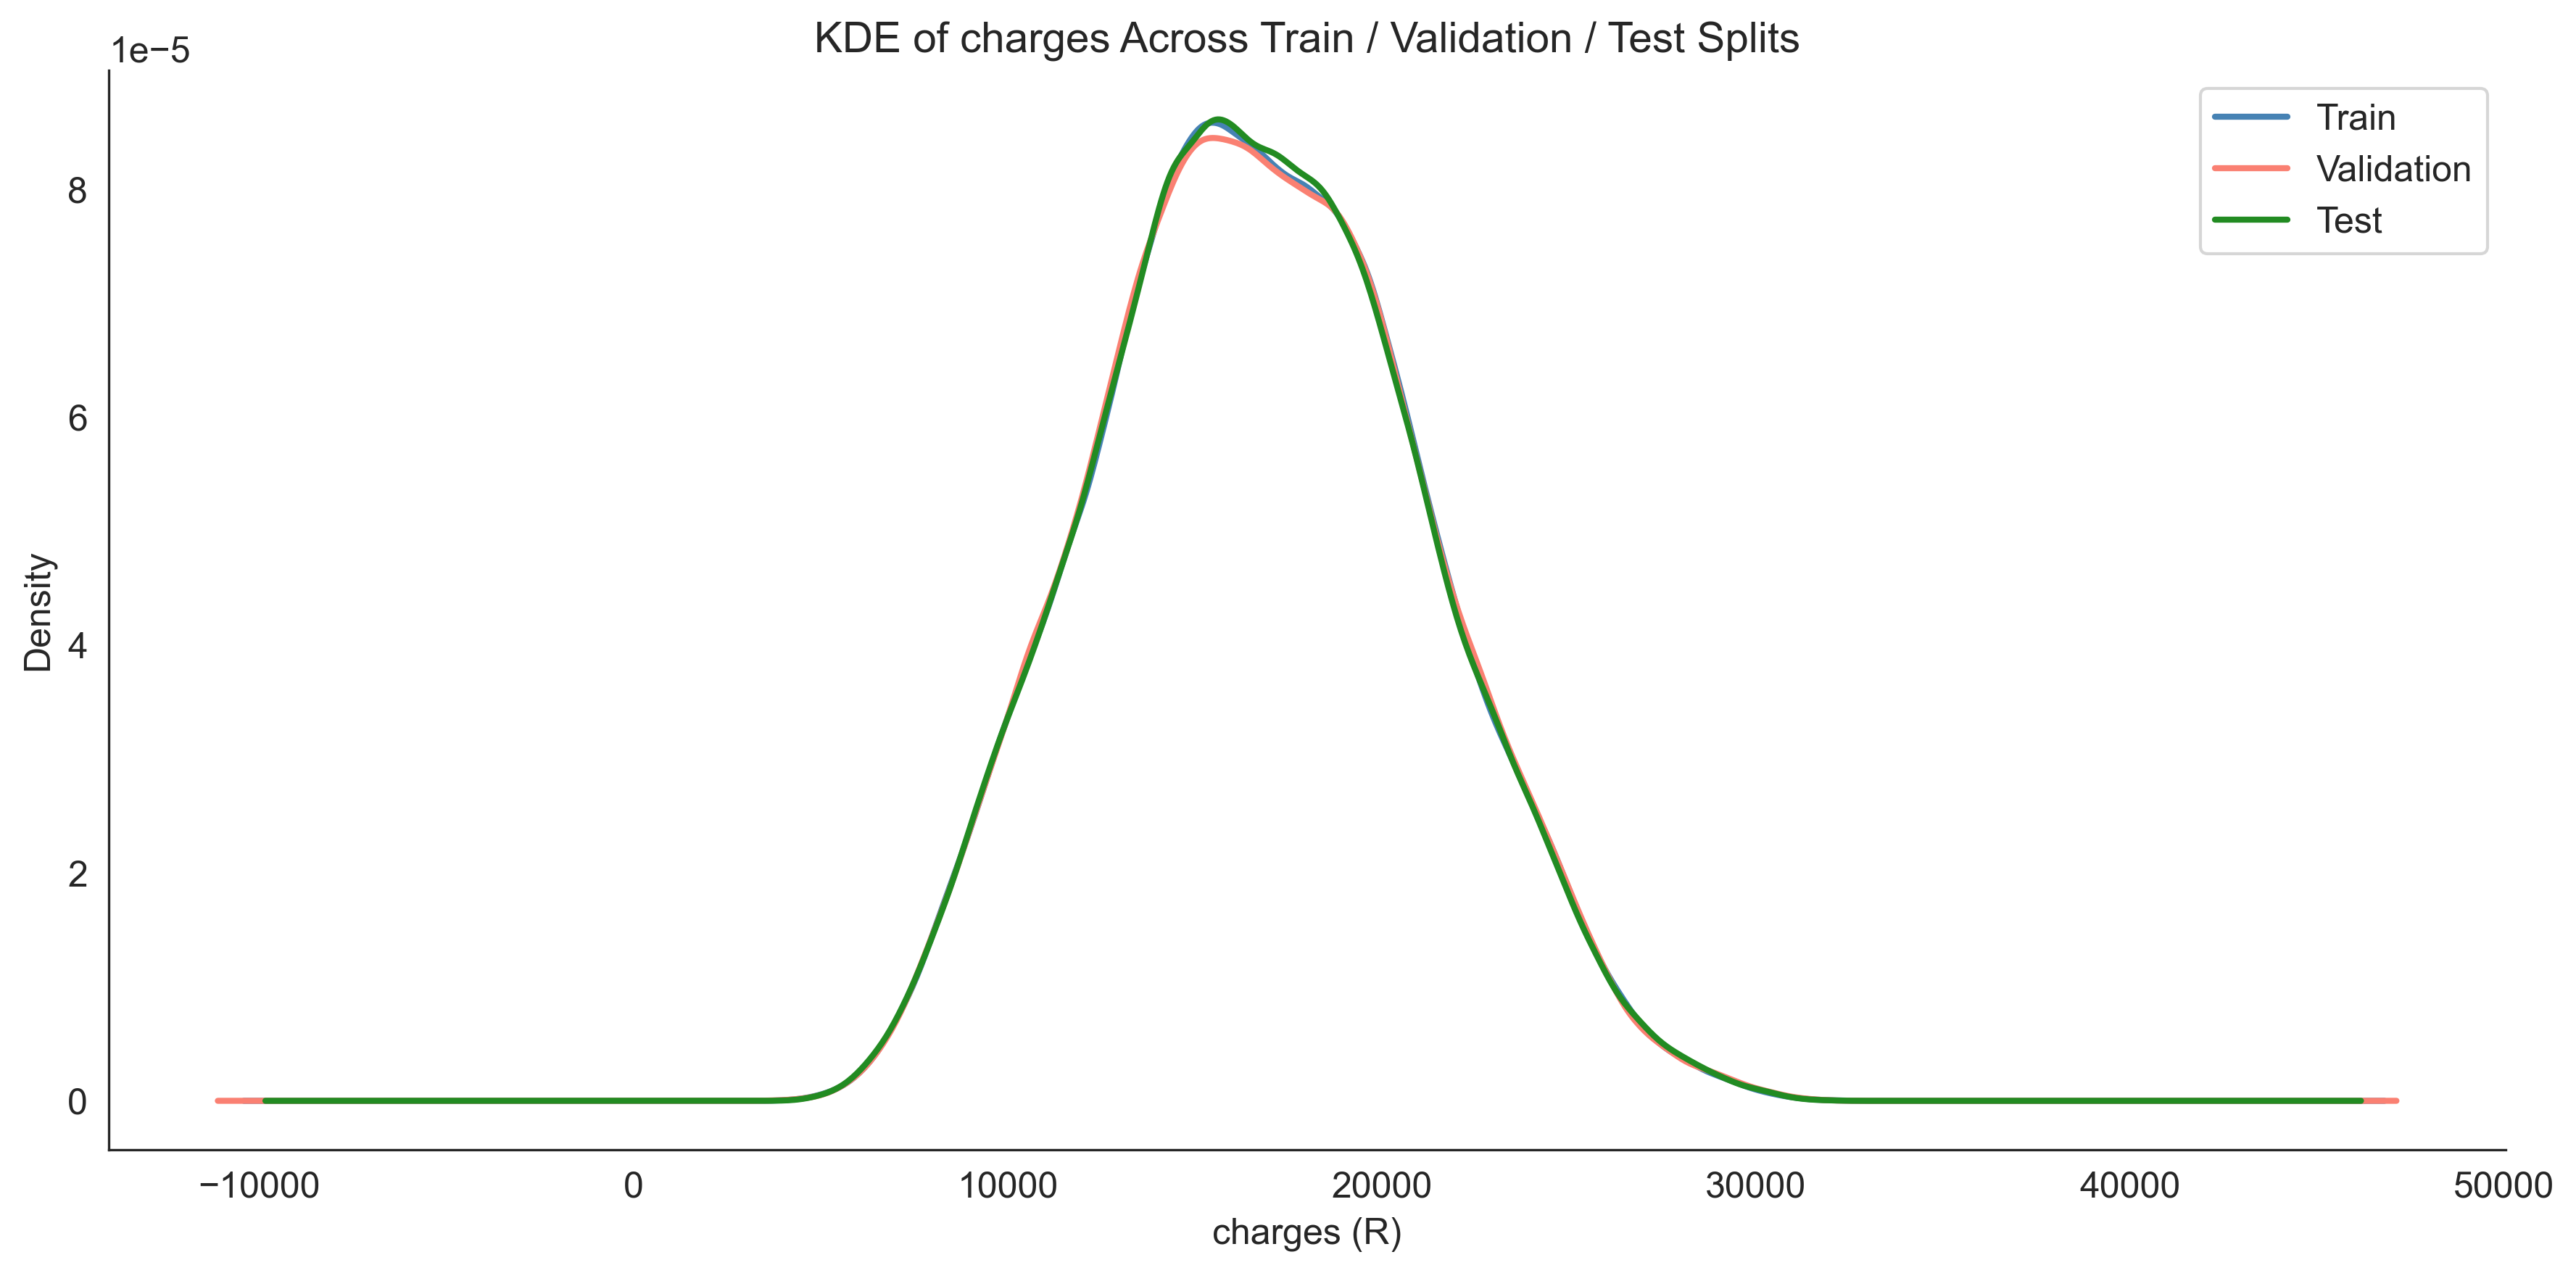
\includegraphics[width=\textwidth]{Thesis/Chapter 4/Figures/fig_split_charges_kde.png}
    \caption{Charges KDE across partitions.}
    \label{fig:annexure_split_charges}
\end{figure}

\begin{figure}[H]
    \centering
    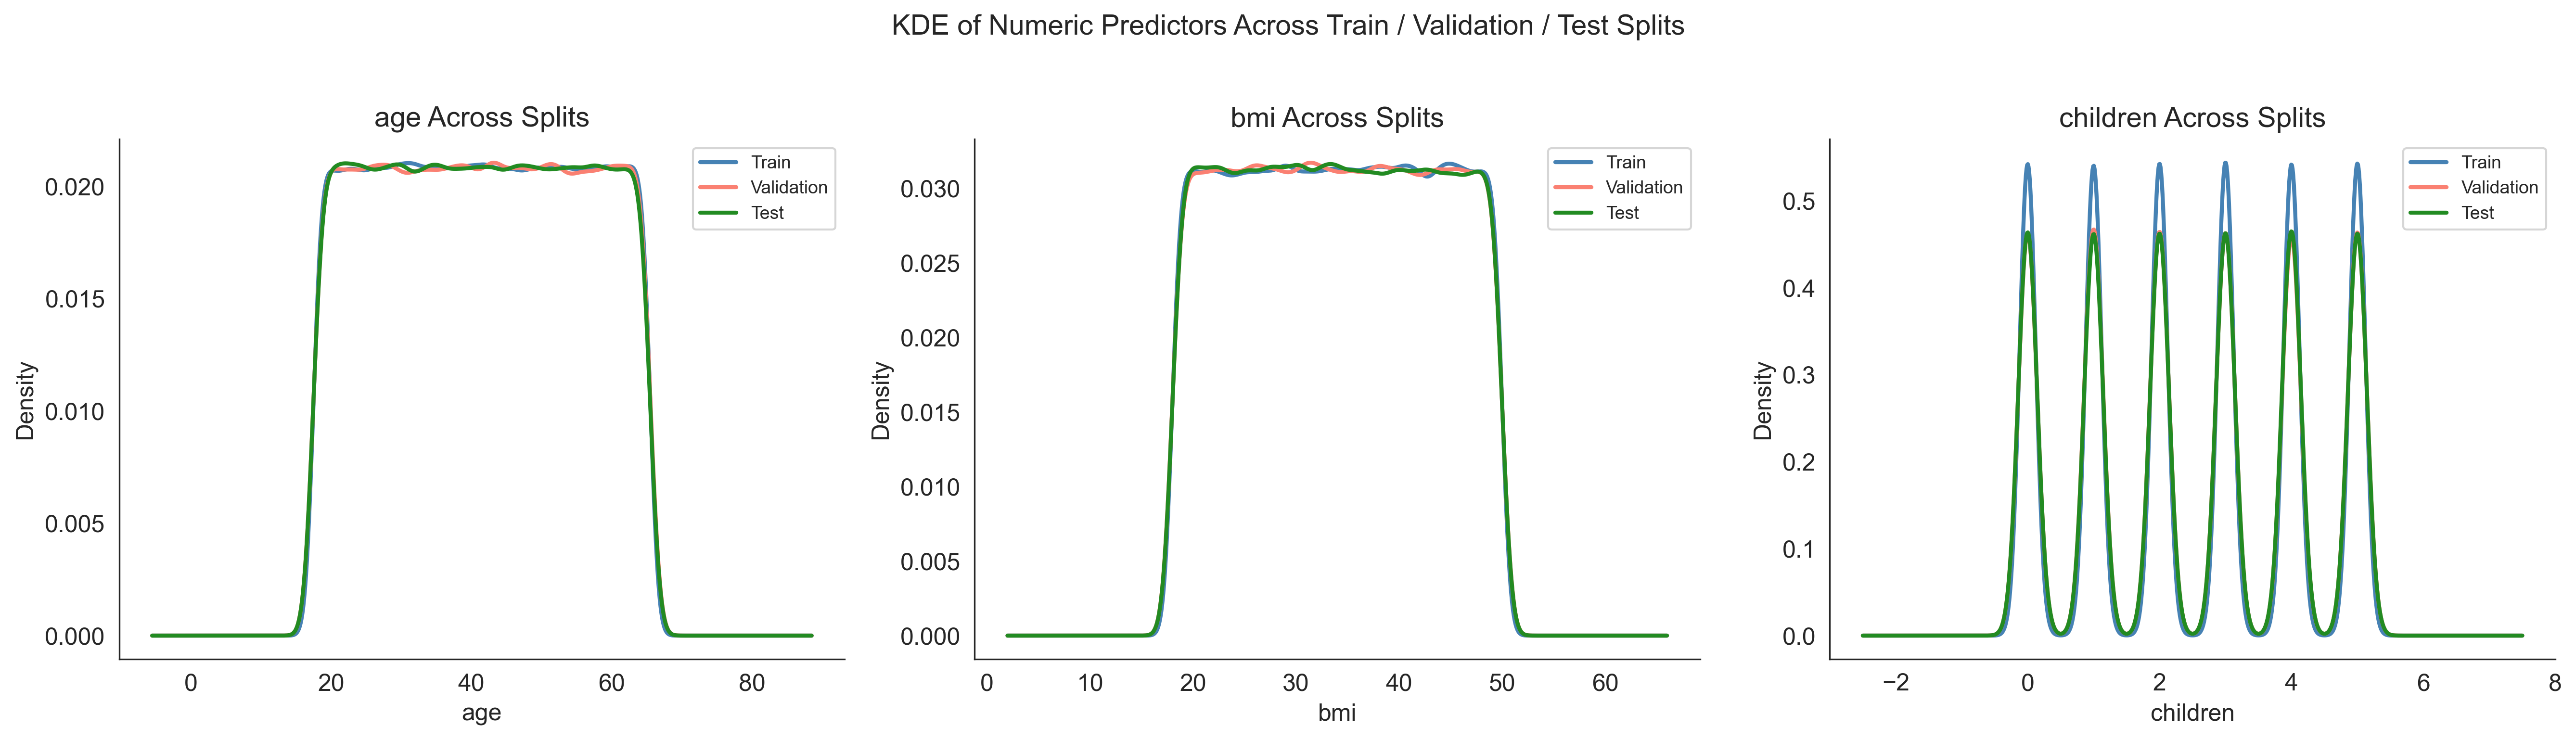
\includegraphics[width=\textwidth]{Thesis/Chapter 4/Figures/fig_split_numeric_kde.png}
    \caption{Numeric feature KDE across partitions.}
    \label{fig:annexure_split_numeric}
\end{figure}

\begin{figure}[H]
    \centering
    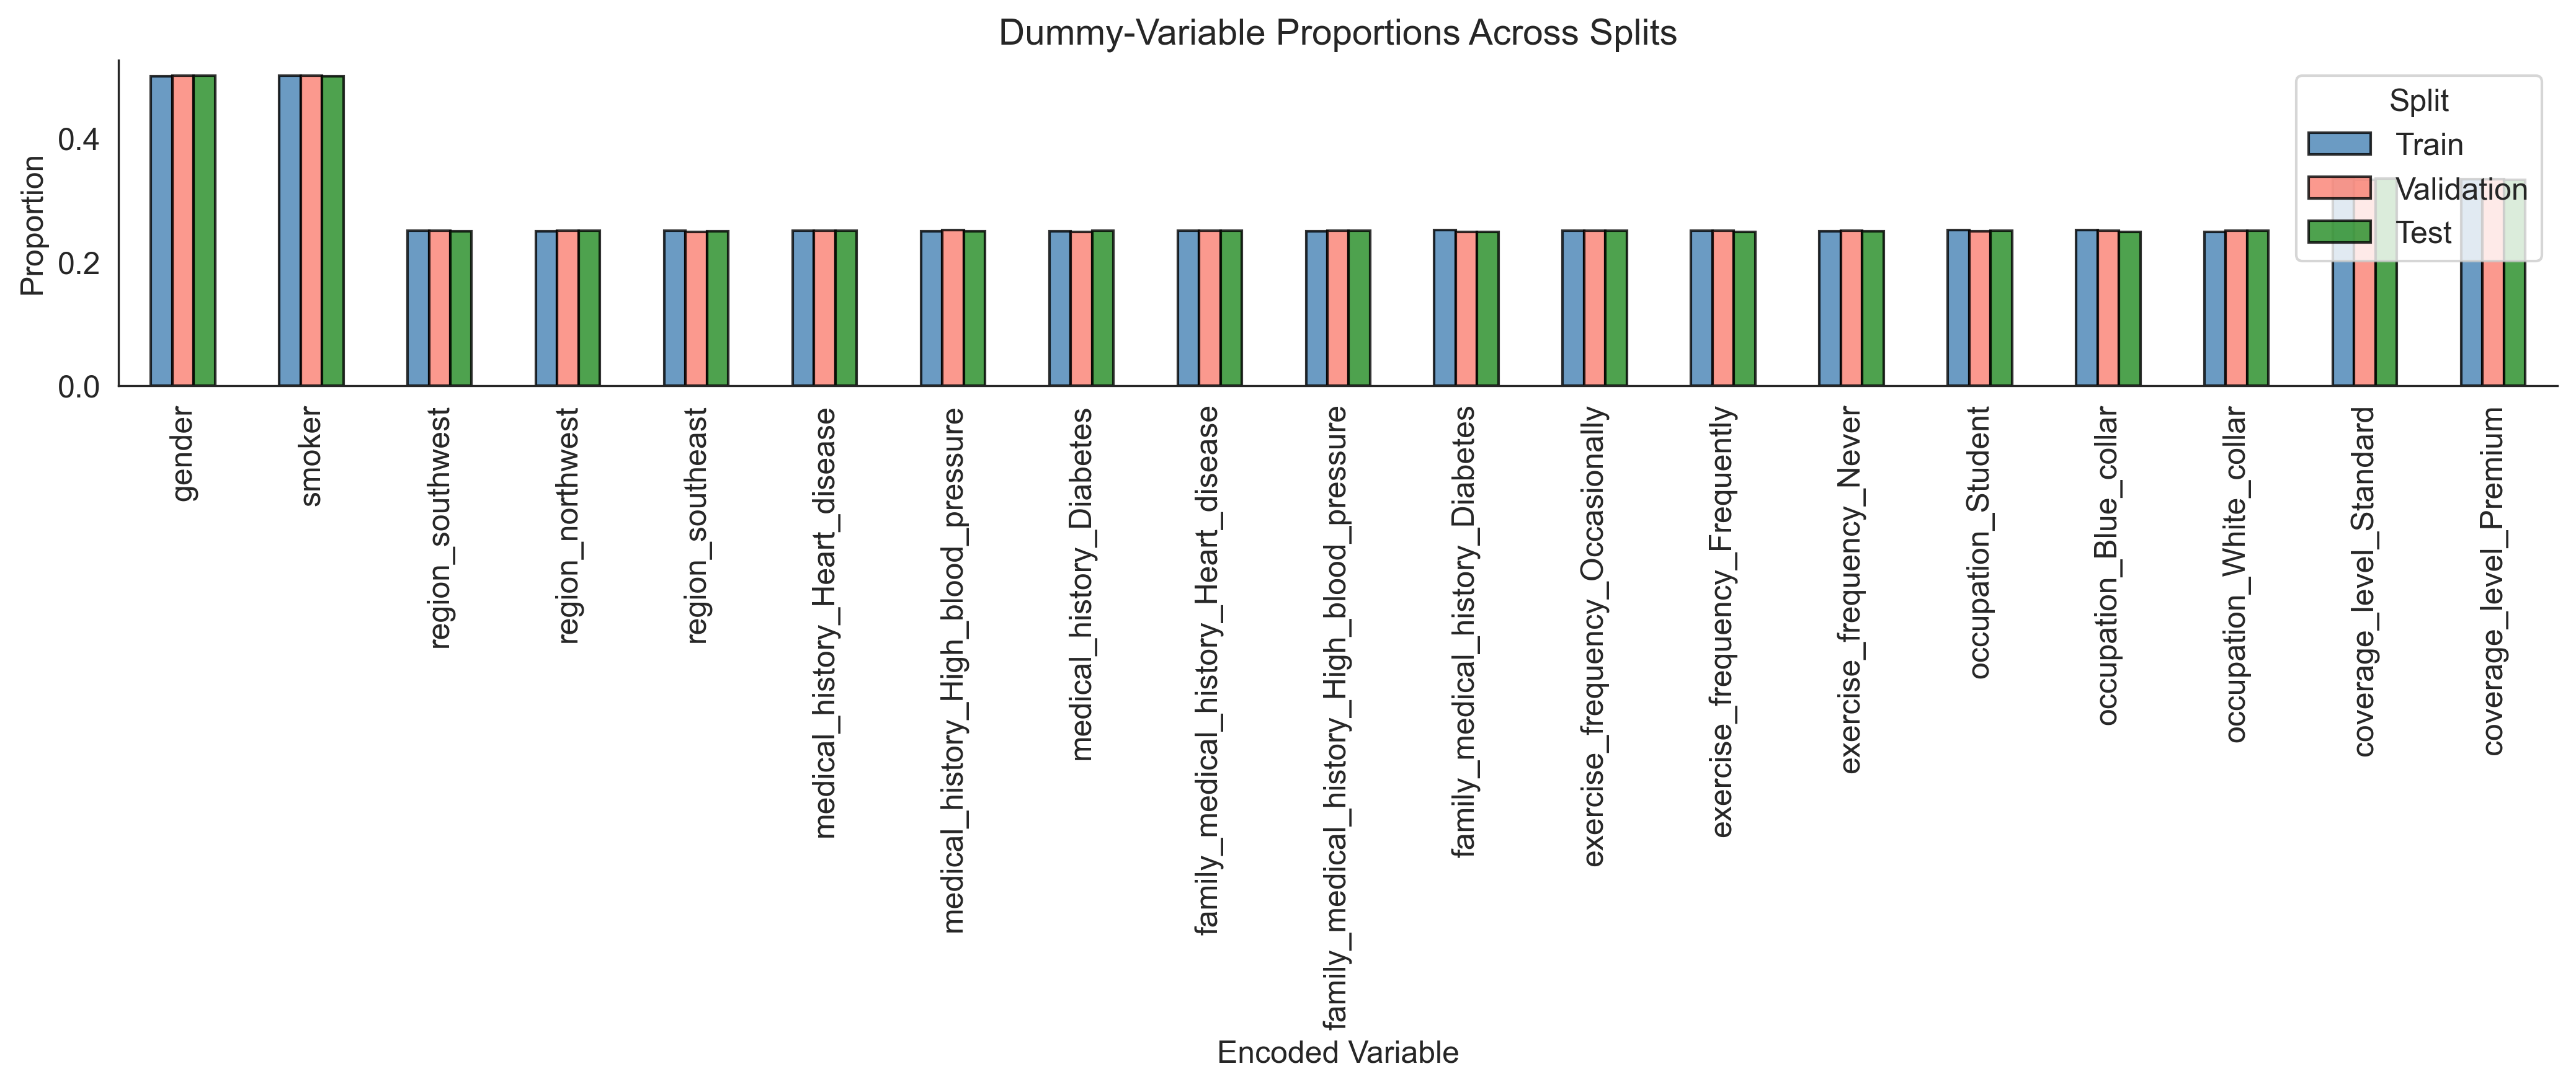
\includegraphics[width=\textwidth]{Thesis/Chapter 4/Figures/fig_split_dummy_proportions.png}
    \caption{Dummy variable proportions across partitions.}
    \label{fig:annexure_split_dummies}
\end{figure}


\clearpage
% =============================================================
% Annexure H: Full Hyperparameter Grid Results
% =============================================================
\section{Full Hyperparameter Grid Results}
\label{annexure:hyperparameters}

% -------------------------------------------------------------
\subsection{Five-Phase Sequential Comparison}
\label{annexure:five_phase}

Hyperparameters were selected through a five-phase sequential comparison procedure. In each phase, one hyperparameter was varied while all others were held at their current best values. The phases proceeded in the following order:

\begin{enumerate}
    \item Activation function (CELU, GELU, Tanh), with fixed lr${}=0.001$, batch size${}=256$, Adam.
    \item Learning rate ($0.01, 0.001, 0.0005, 0.0001$), with fixed best activation, batch size${}=256$, Adam.
    \item Batch size ($64, 128, 256, 512$), with fixed best activation and learning rate, Adam.
    \item Optimiser (Adam vs NAdam), with all previous best values fixed.
    \item Momentum $\beta_1$ ($0.90, 0.95, 0.99$) with $\beta_2 = 0.999$ fixed, using the best optimiser.
\end{enumerate}

Each configuration was trained with early stopping (patience of 10 validation checks at 5-epoch intervals) up to a maximum of 100 epochs. Table~\ref{tab:hyper_full} reports the full results.

\begin{table}[htbp]
\centering
\caption{Full five-phase hyperparameter comparison results.}
\label{tab:hyper_full}
\footnotesize
\begin{tabular}{llrrr}
\toprule
\textbf{Phase} & \textbf{Configuration} & \textbf{Best Epoch} & \textbf{Val $R^2$} & \textbf{Time (s)} \\
\midrule
\multirow{3}{*}{Phase 1: Activation}
  & CELU  & 100 & 0.995682 & 556.7 \\
  & GELU  &  25 & 0.995636 & 313.8 \\
  & Tanh  & 100 & 0.995532 & 565.9 \\
\midrule
\multirow{4}{*}{Phase 2: Learning Rate}
  & 0.01   &  10 & 0.995453 & 222.9 \\
  & 0.001  & 100 & 0.995682 & 558.1 \\
  & 0.0005 & 100 & 0.995692 & 563.8 \\
  & 0.0001 & 100 & 0.995686 & 556.0 \\
\midrule
\multirow{4}{*}{Phase 3: Batch Size}
  & 64  &  75 & 0.995678 & 1441.8 \\
  & 128 &  30 & 0.995669 &  491.9 \\
  & 256 & 100 & 0.995692 &  580.3 \\
  & 512 & 160 & 0.995685 &  487.3 \\
\midrule
\multirow{2}{*}{Phase 4: Optimiser}
  & Adam  & 100 & 0.995692 & 562.7 \\
  & NAdam &  85 & 0.995693 & 582.5 \\
\midrule
\multirow{3}{*}{Phase 5: Momentum}
  & $\beta_1=0.90$ & 85 & 0.995693 & 586.6 \\
  & $\beta_1=0.95$ & 40 & 0.995690 & 427.8 \\
  & $\beta_1=0.99$ & 95 & 0.995685 & 621.8 \\
\bottomrule
\end{tabular}
\end{table}

% -------------------------------------------------------------
\subsection{Phase Comparison Figures}
\label{annexure:phase_figures}

The following figures present the validation MSE loss and validation $R^2$
trajectories for each phase of the sequential hyperparameter comparison.

\begin{figure}[H]
\centering
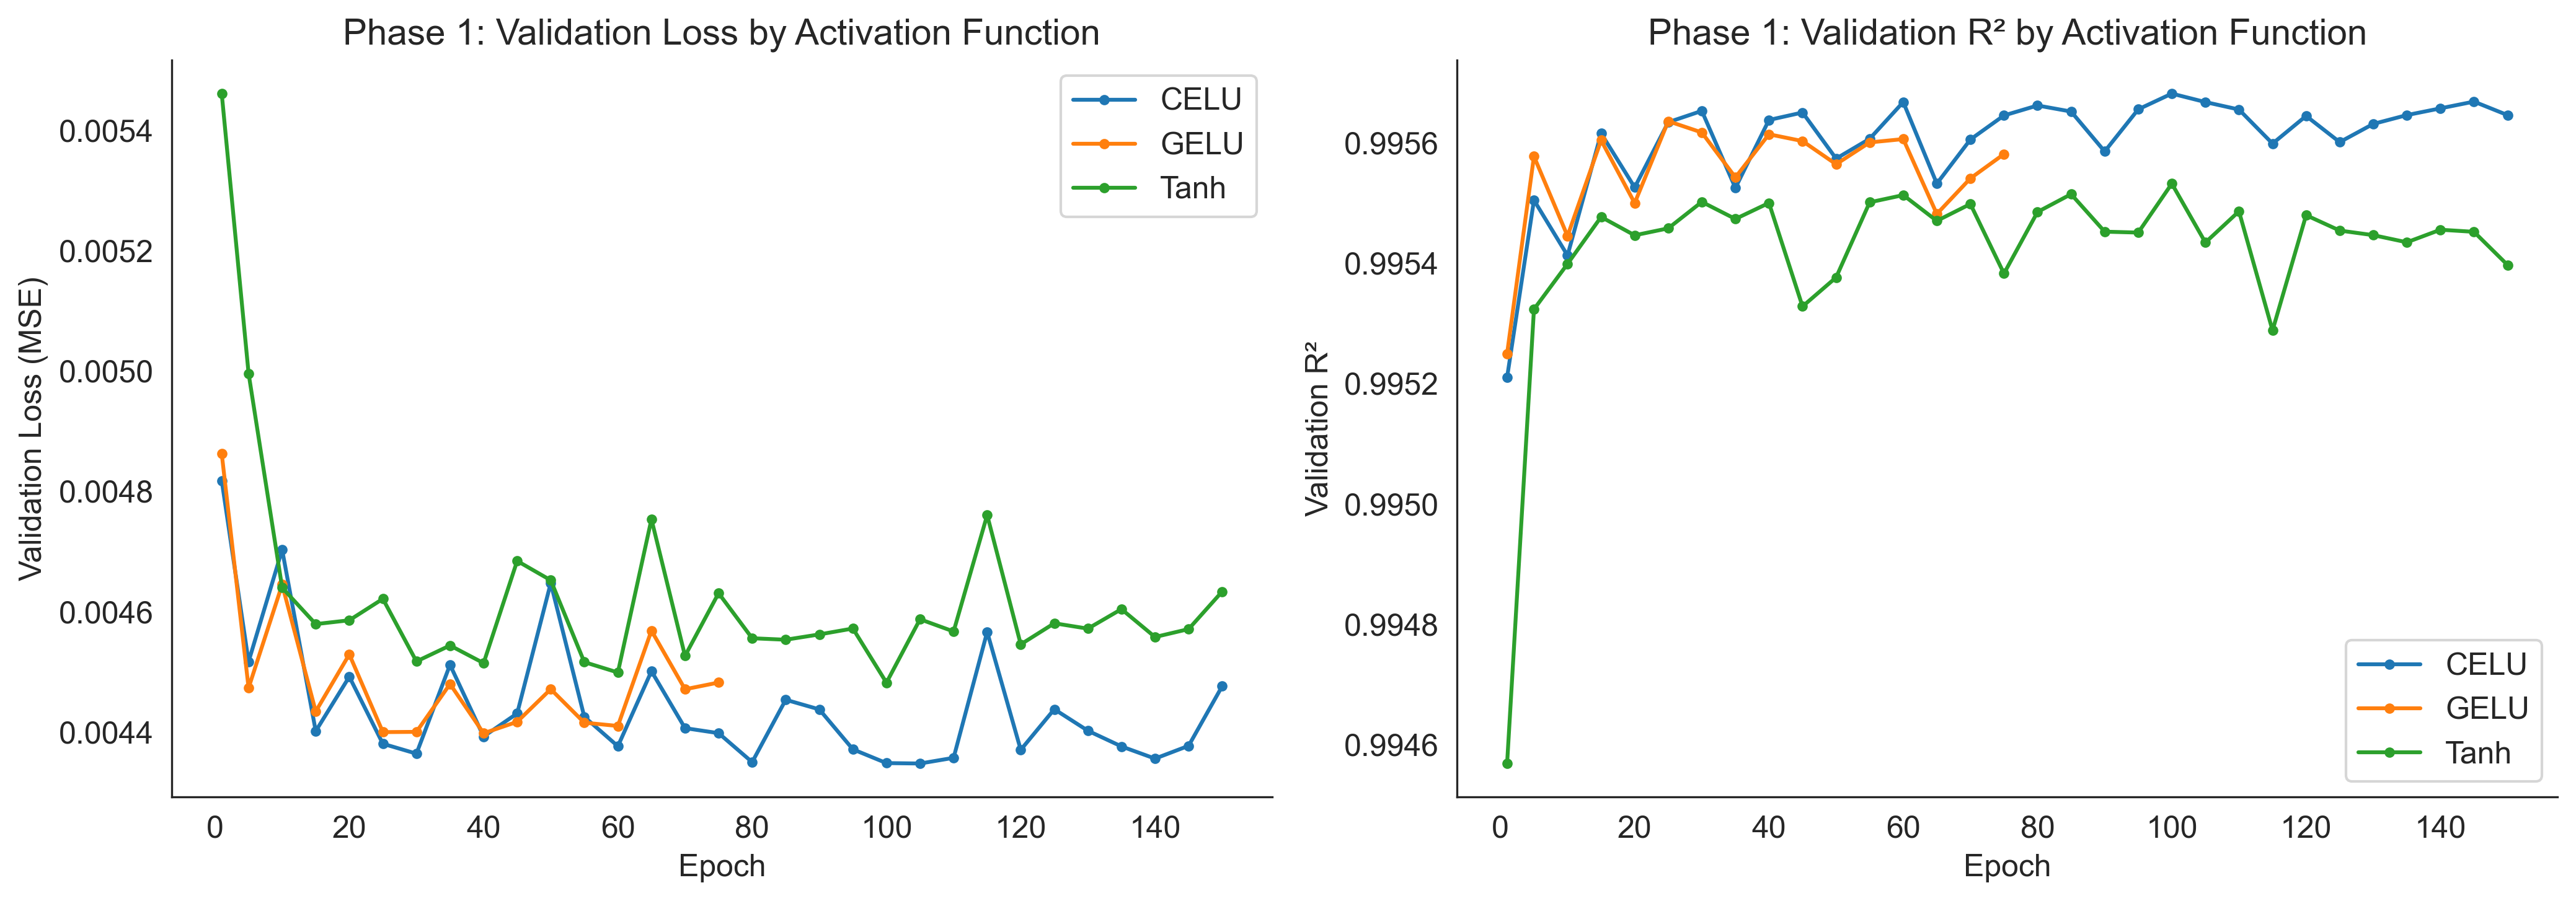
\includegraphics[width=0.95\textwidth]{Thesis/Chapter 4/Figures/fig_phase1_activation_comparison.png}
\caption{Phase~1: validation MSE loss (left) and validation $R^2$
(right) by activation function over training epochs.}
\label{fig:phase1_activation_annex}
\end{figure}

\begin{figure}[H]
\centering
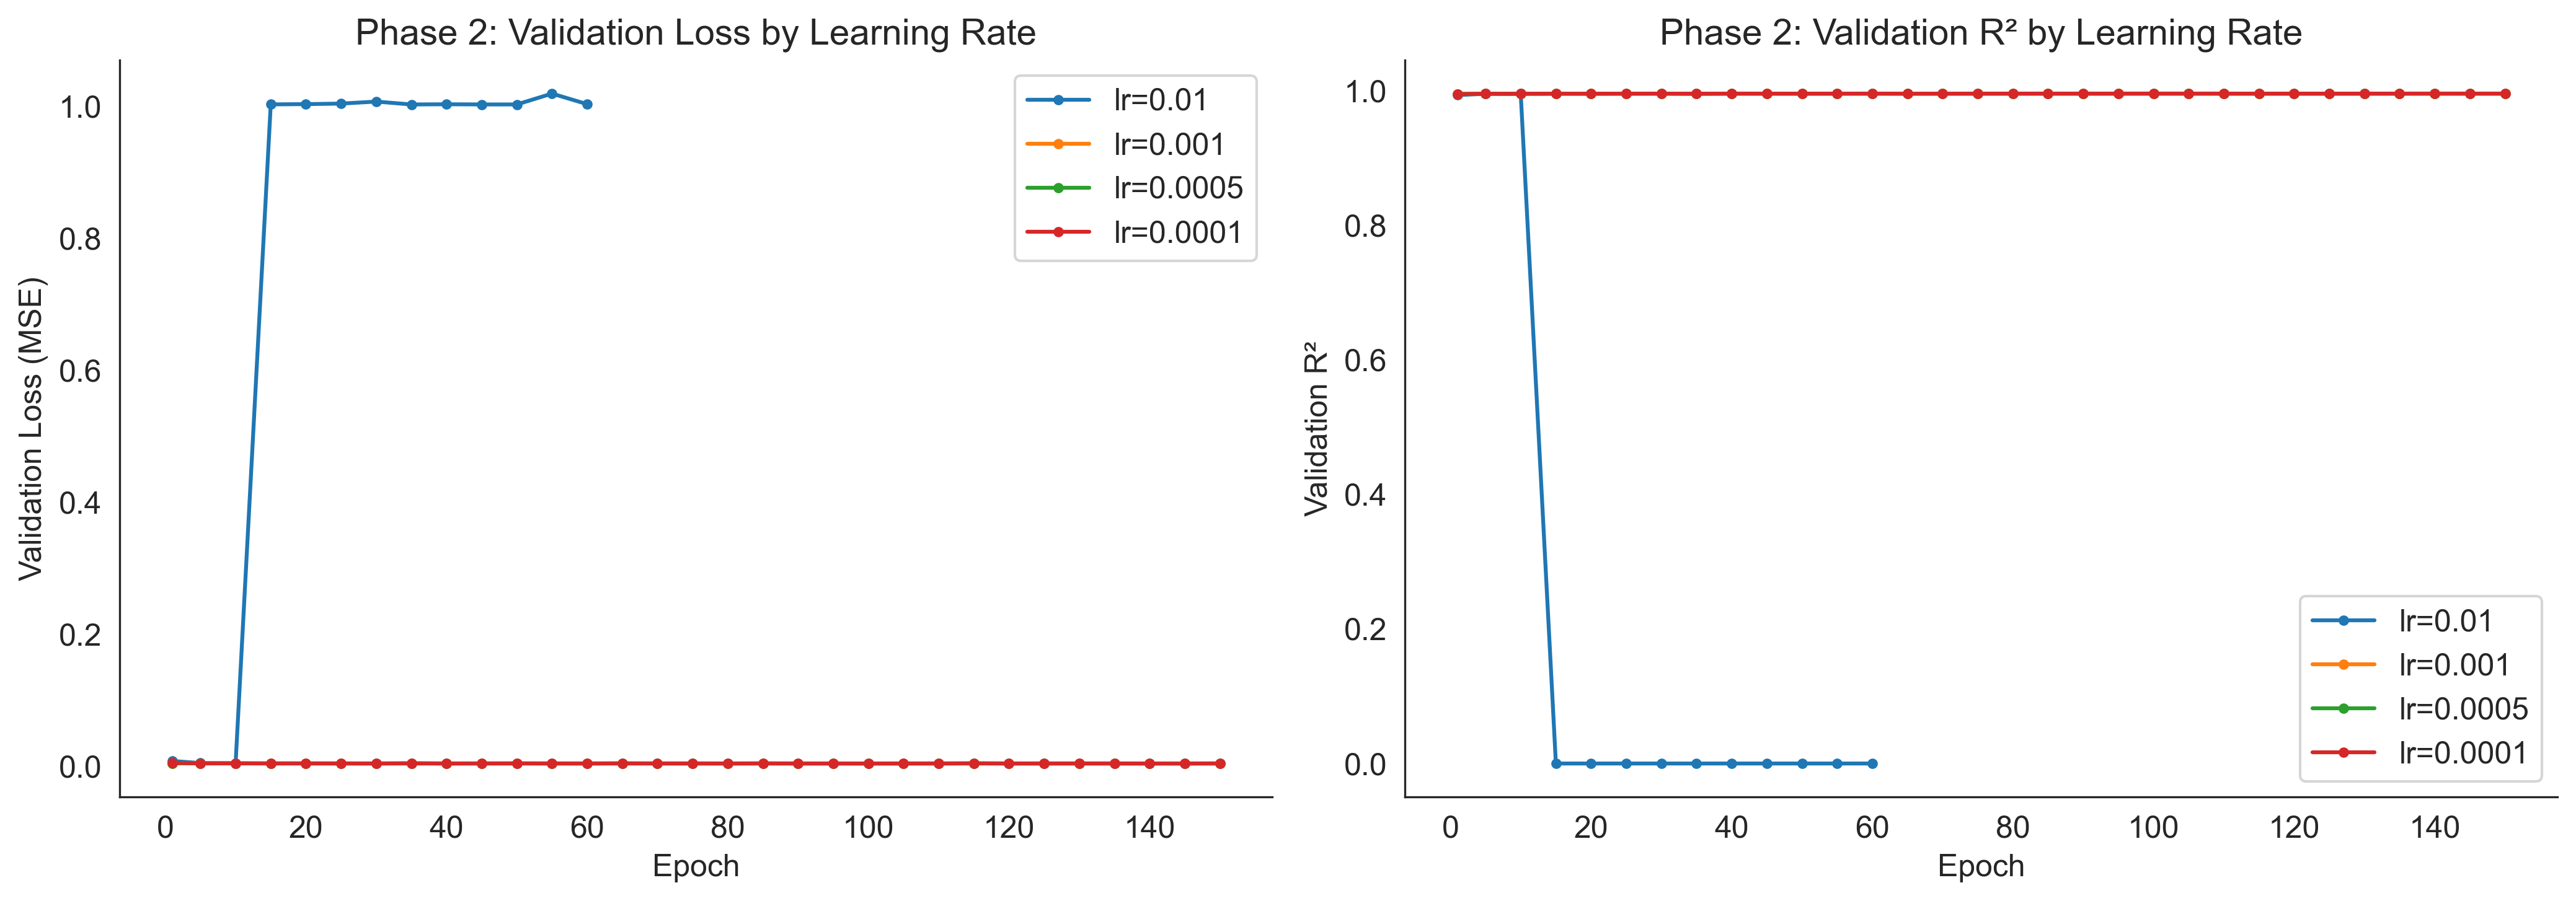
\includegraphics[width=0.95\textwidth]{Thesis/Chapter 4/Figures/fig_phase2_lr_comparison.png}
\caption{Phase~2: validation MSE loss (left) and validation $R^2$
(right) by learning rate.}
\label{fig:phase2_lr_annex}
\end{figure}

\begin{figure}[H]
\centering
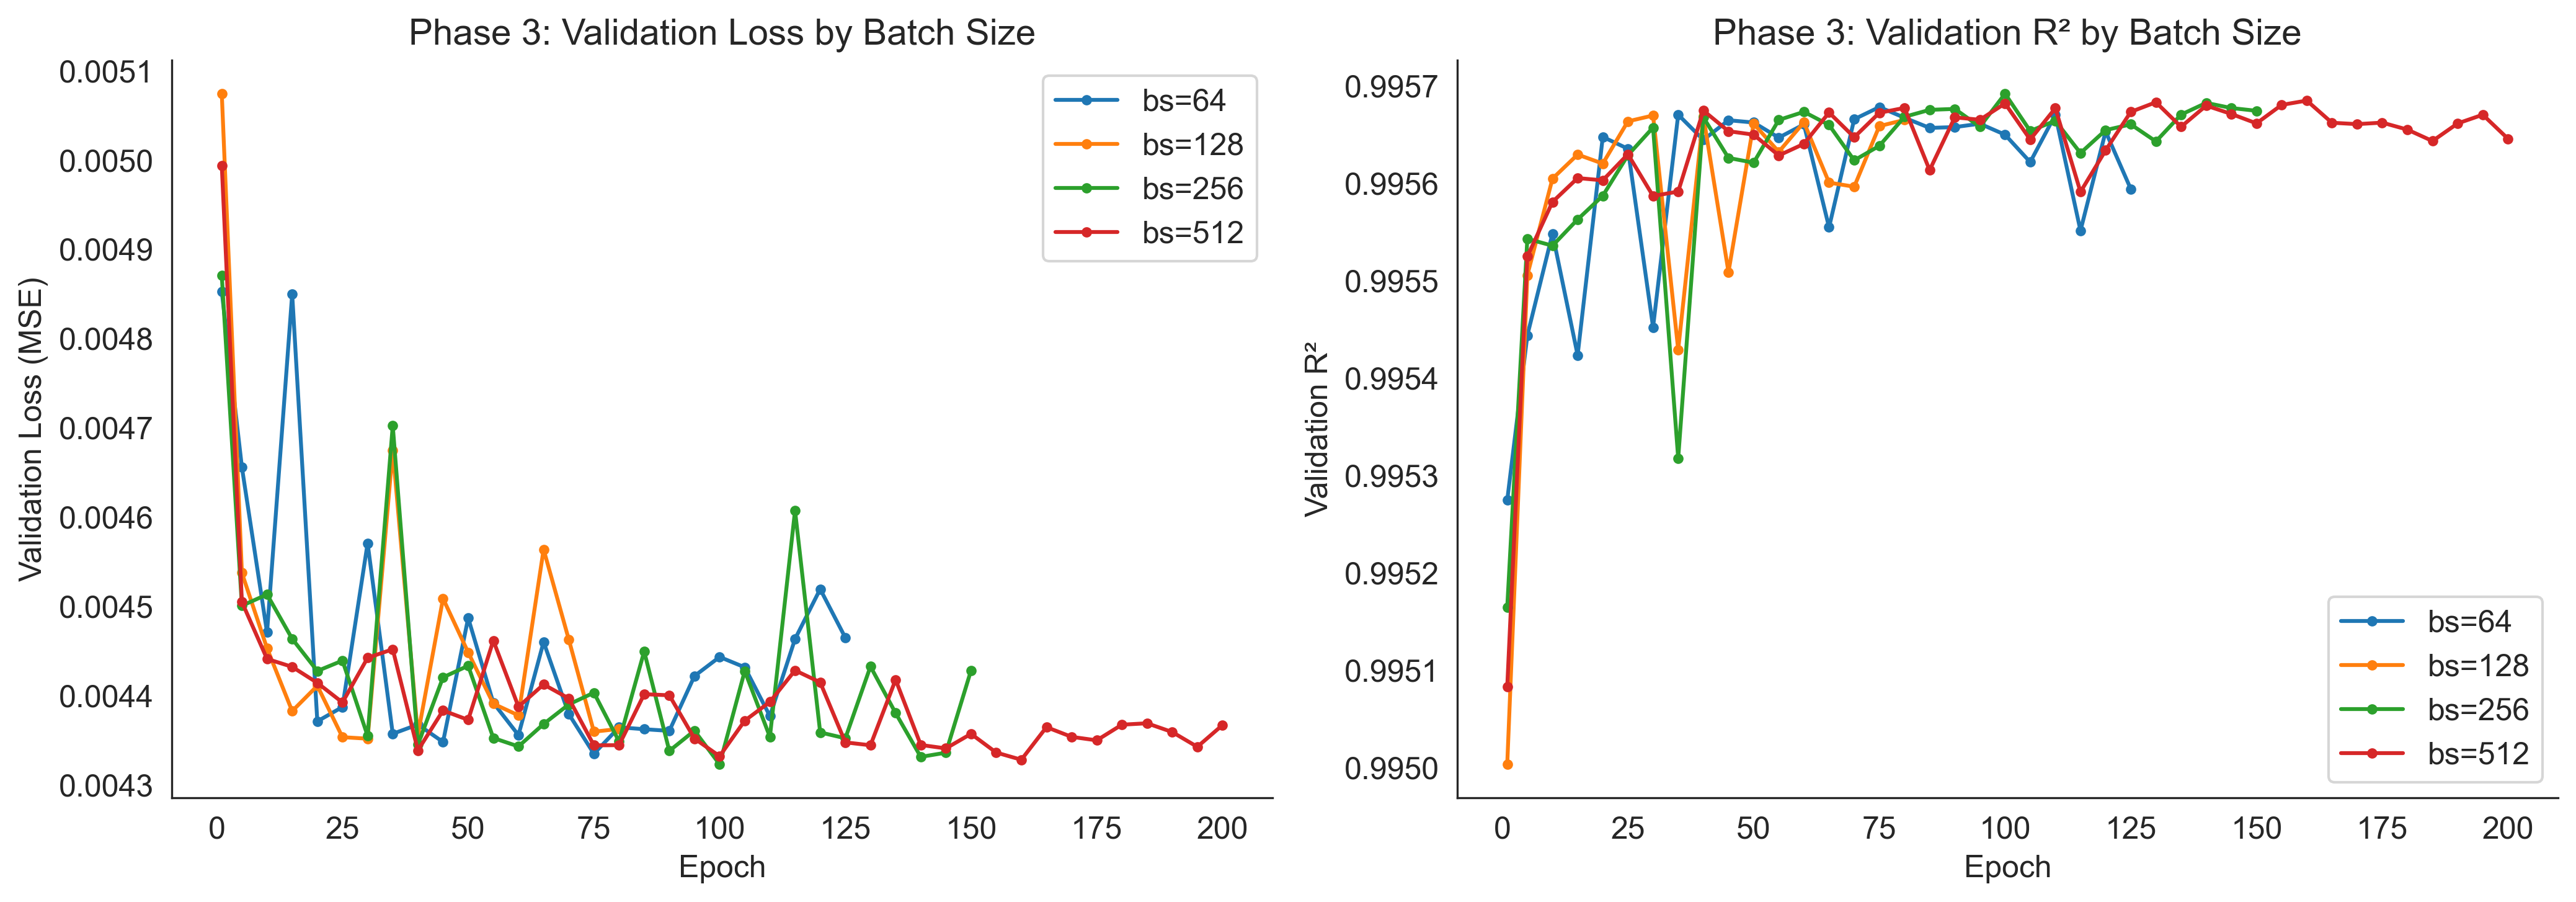
\includegraphics[width=0.95\textwidth]{Thesis/Chapter 4/Figures/fig_phase3_batchsize_comparison.png}
\caption{Phase~3: validation MSE loss (left) and validation $R^2$
(right) by batch size.}
\label{fig:phase3_batchsize_annex}
\end{figure}

\begin{figure}[H]
\centering
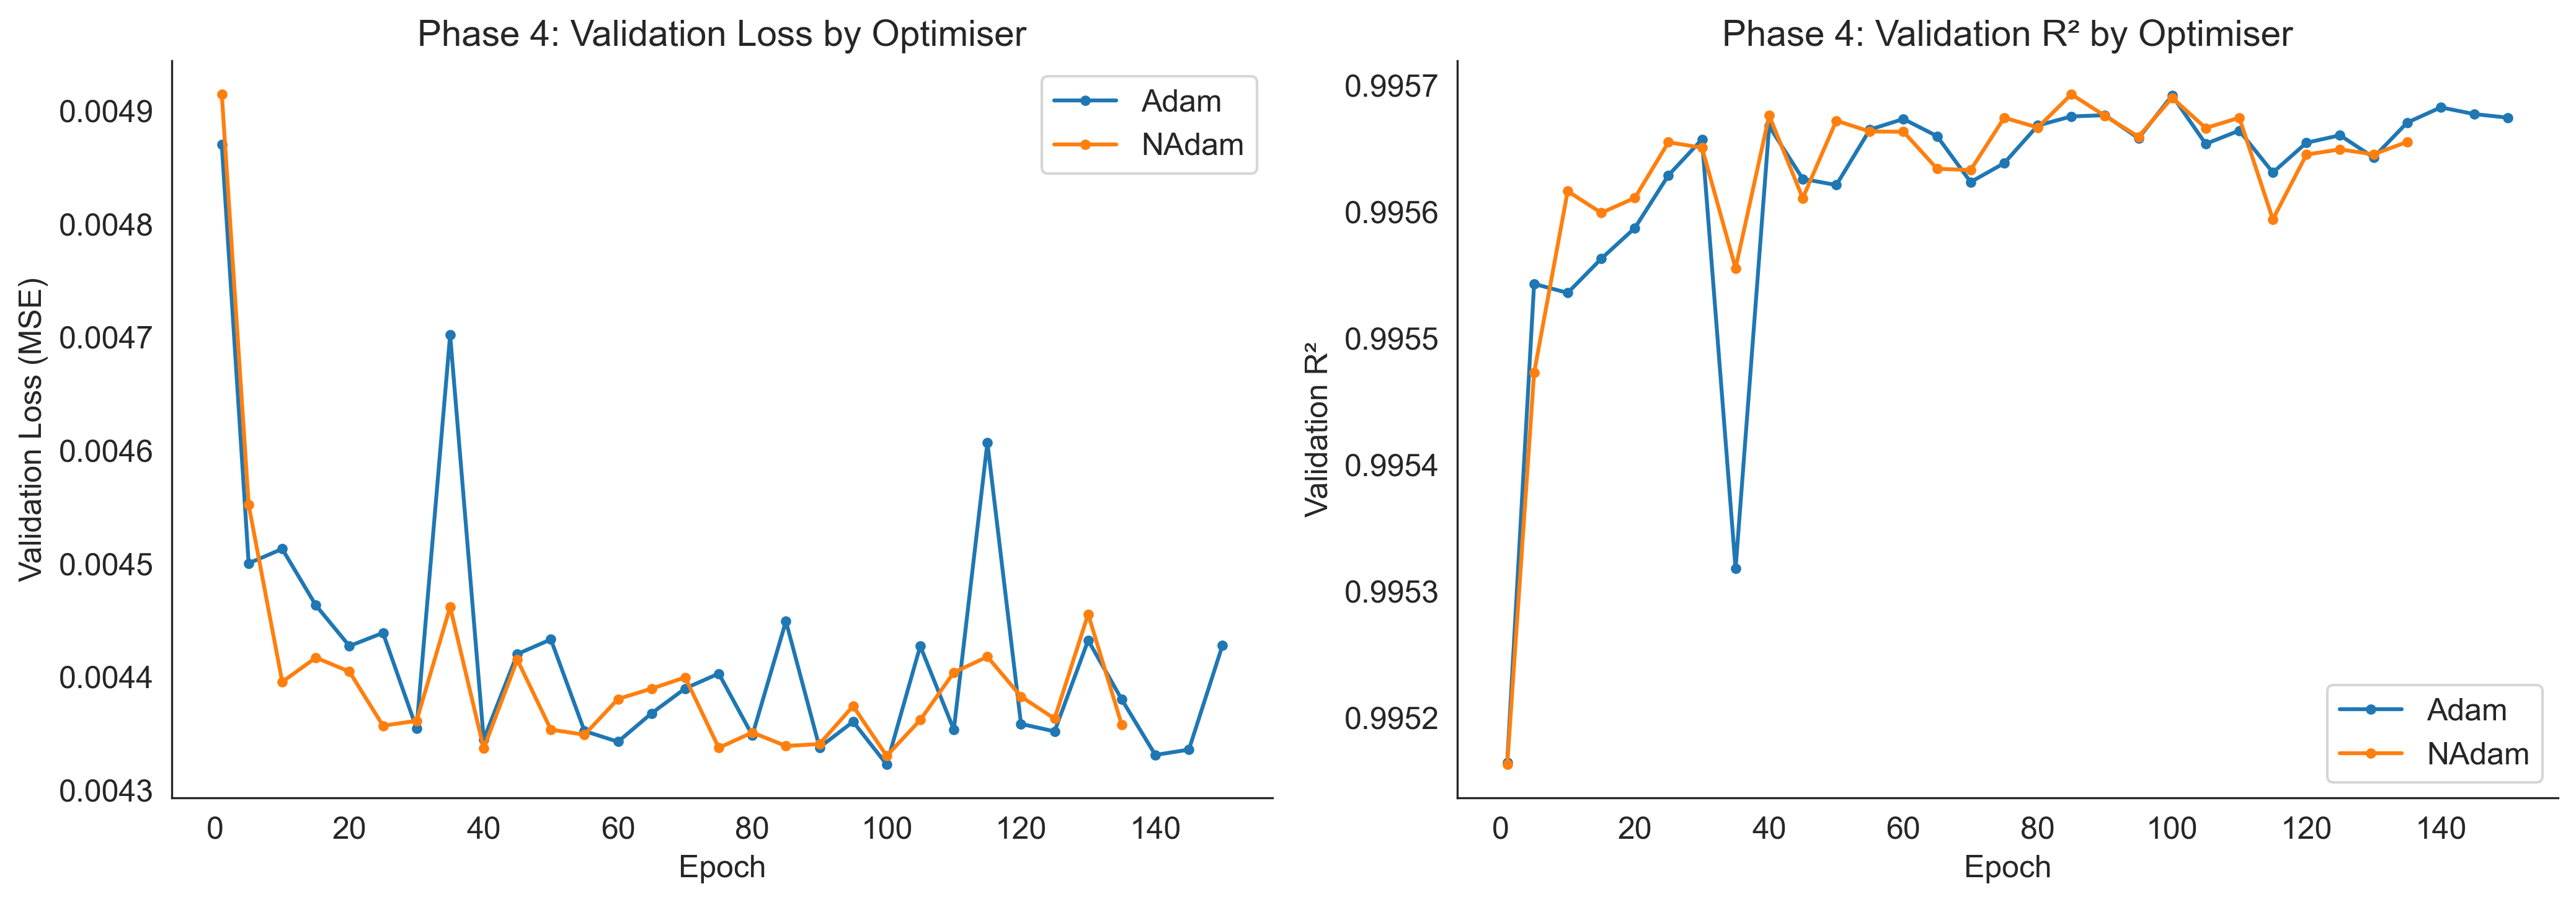
\includegraphics[width=0.95\textwidth]{Thesis/Chapter 4/Figures/fig_phase4_optimiser_comparison.png}
\caption{Phase~4: validation MSE loss (left) and validation $R^2$
(right) by optimiser.}
\label{fig:phase4_optimiser_annex}
\end{figure}

\begin{figure}[H]
\centering
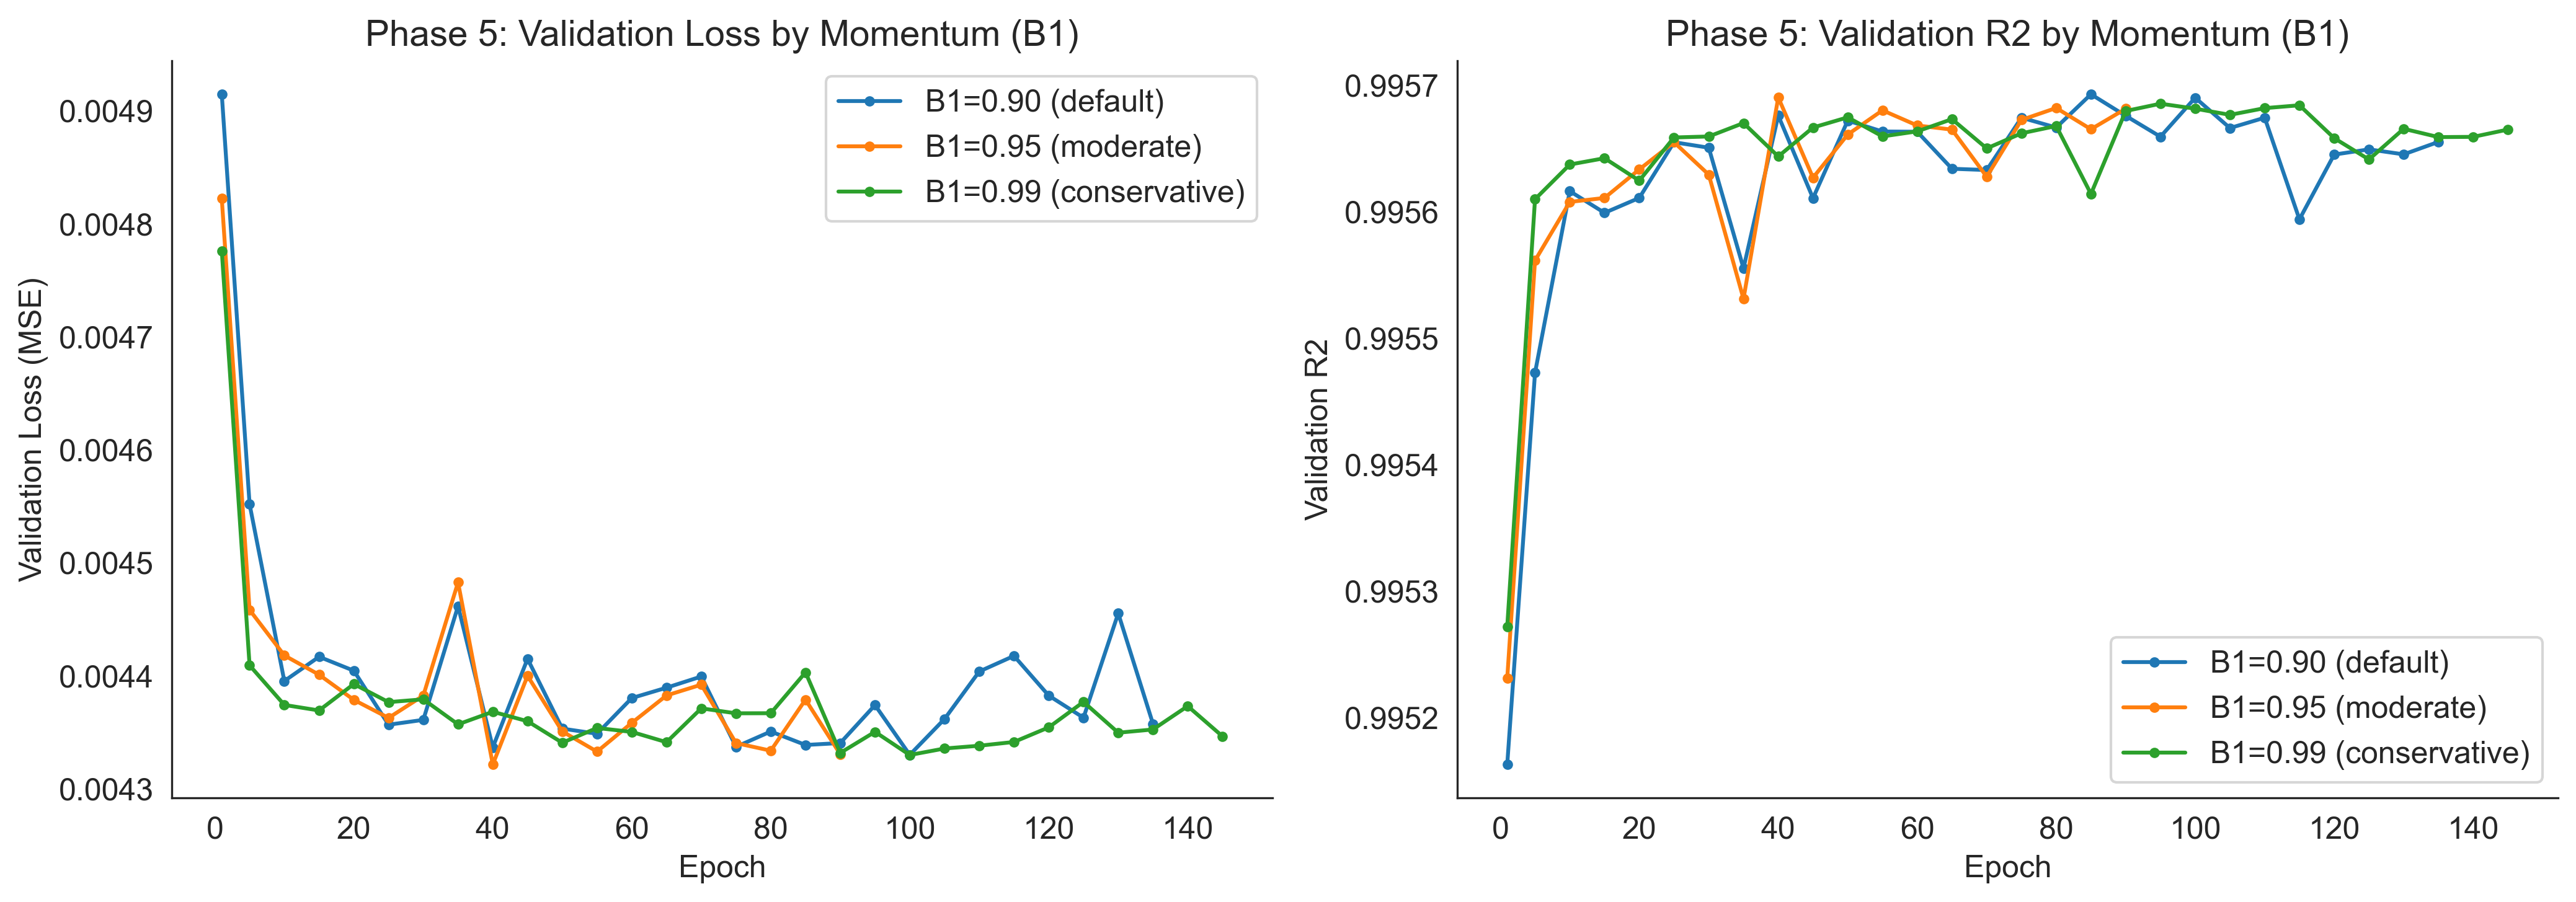
\includegraphics[width=0.95\textwidth]{Thesis/Chapter 4/Figures/fig_phase5_momentum_comparison.png}
\caption{Phase~5: validation MSE loss (left) and validation $R^2$
(right) by first momentum coefficient $\beta_1$.}
\label{fig:phase5_momentum_annex}
\end{figure}

\begin{figure}[H]
\centering
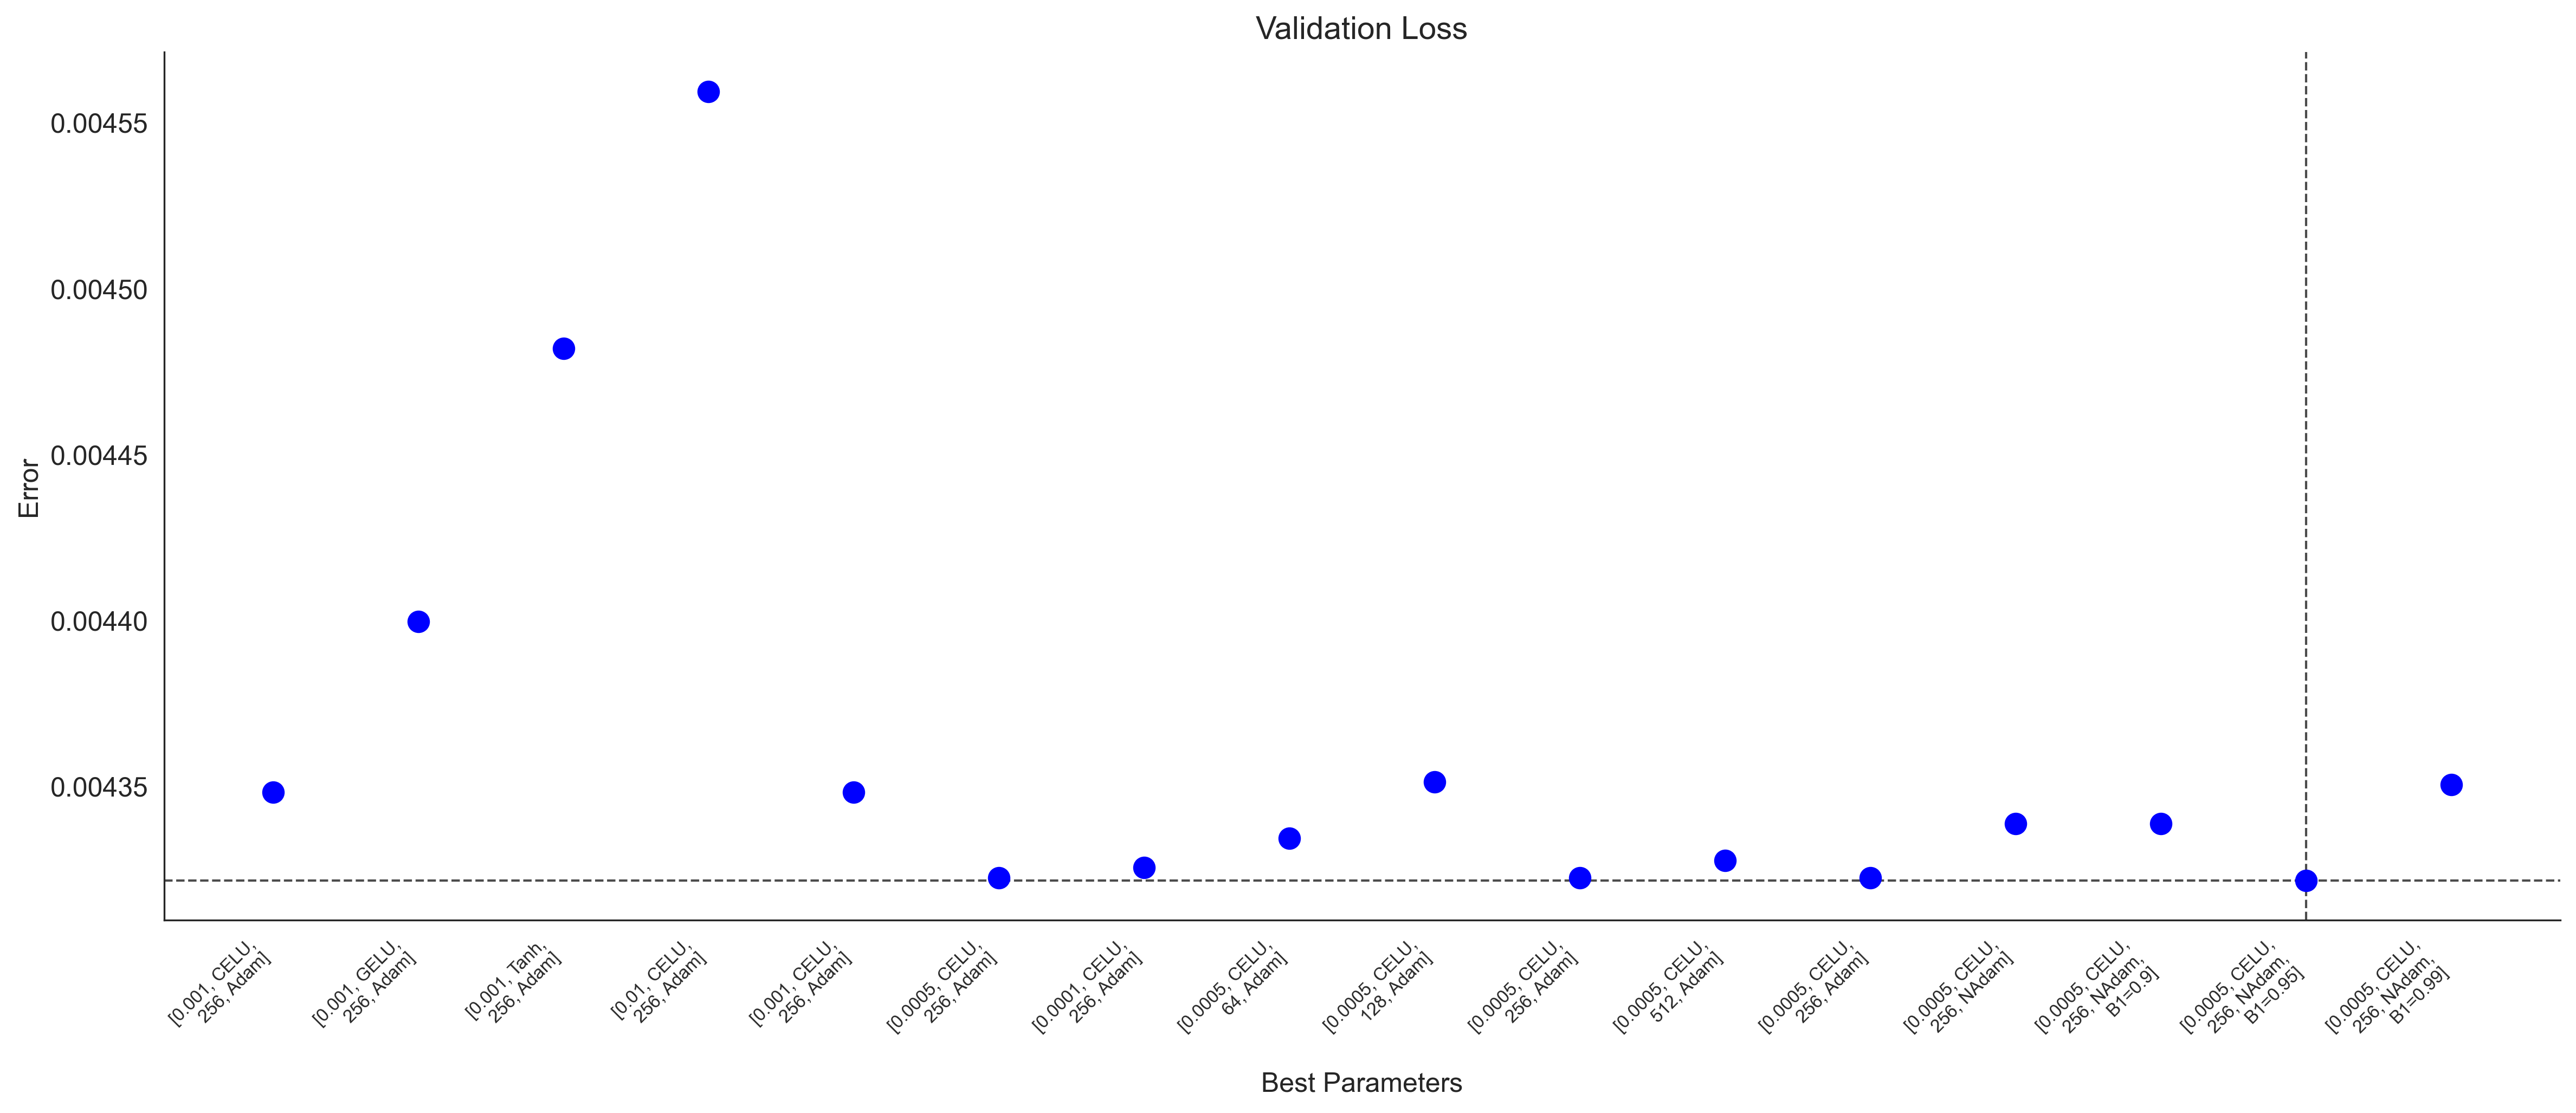
\includegraphics[width=0.95\textwidth]{Thesis/Chapter 4/Figures/fig_validation_loss_hyperparameters.png}
\caption{Best validation MSE loss across all hyperparameter
configurations evaluated in Phases~1 to~5.}
\label{fig:validation_loss_overview_annex}
\end{figure}

% -------------------------------------------------------------
\subsection{Bayesian Optimisation: GP Surrogate}
\label{annexure:bo_methodology}

A Gaussian process surrogate with a Mat\'{e}rn $\nu = 5/2$ kernel was fitted to the observed hyperparameter evaluations to visualise the validation-error landscape. The GP was fitted using scikit-learn's \texttt{GaussianProcessRegressor} with 15 random restarts, seed 42, and a composite kernel consisting of a constant kernel multiplied by the Mat\'{e}rn kernel plus a white noise kernel. Log-scaled axes were used for the learning rate dimension. The fitted surface and its uncertainty were evaluated on a $100 \times 100$ grid with 15\% margin beyond the observed range.

% -------------------------------------------------------------
\subsection{Consolidated Best Hyperparameter Summary}
\label{annexure:best_hyperparams}

\begin{table}[htbp]
\centering
\caption{Best hyperparameter configuration selected for the final DNN model.}
\label{tab:best_hyperparams}
\begin{tabular}{ll}
\toprule
\textbf{Hyperparameter} & \textbf{Selected Value} \\
\midrule
Architecture    & $22 \to 256 \to 128 \to 64 \to 32 \to 16 \to 1$ \\
Activation      & CELU \\
Learning rate   & 0.0005 \\
Batch size      & 256 \\
Optimiser       & NAdam \\
$\beta_1$       & 0.90 \\
$\beta_2$       & 0.999 \\
Bias            & False (all layers) \\
Max epochs      & 100 \\
Early stopping  & 10 checks (every 5 epochs) \\
Loss function   & MSE (on normalised scale) \\
\bottomrule
\end{tabular}
\end{table}



\clearpage
% =============================================================
% Annexure I: Software and Environment Details
% =============================================================
\section{Software and Environment Details}
\label{annexure:software}


% -------------------------------------------------------------
\subsection{Python Distribution and Version}
\label{annexure:python}

Python~3.11 via the Anaconda distribution. Jupyter Notebook was used for interactive development.

% -------------------------------------------------------------
\subsection{Core Package Versions}
\label{annexure:packages}

\begin{table}[htbp]
\centering
\caption{Python package versions used in the dissertation.}
\label{tab:packages}
\begin{tabular}{lll}
\hline
\textbf{Package} & \textbf{Version} & \textbf{Purpose} \\
\hline
PyTorch           & 2.x              & DNN architecture, training and inference \\
SHAP              & 0.43+            & Shapley value computation (GradientExplainer) \\
statsmodels       & 0.14+            & GLM (Gamma, log-link) fitting \\
NumPy             & 1.24+            & Numerical computation \\
pandas            & 2.x              & Data manipulation and I/O \\
SciPy             & 1.11+            & Statistical tests, distributions \\
scikit-learn      & 1.3+             & GP surrogate, train/test splitting, metrics \\
matplotlib        & 3.8+             & Static figure generation \\
seaborn           & 0.13+            & Statistical visualisation \\
scikit-optimize   & 0.10+            & Bayesian Optimisation (\texttt{gp\_minimize}) \\
Plotly            & 5.x              & Interactive 3D surface plots \\
\hline
\end{tabular}

\medskip
\emph{Note:} Exact patch versions may vary. The versions above represent the minimum versions with which the code was tested. Update these entries with the output of \texttt{pip freeze} or \texttt{conda list} before final submission.
\end{table}

% -------------------------------------------------------------
\subsection{Hardware Platform}
\label{annexure:hardware}

\begin{itemize}
    \item Processor: Apple Silicon (M-series)
    \item Primary compute device: MPS (Metal Performance Shaders) via PyTorch
    \item SHAP compute device: CPU (faster than MPS for GradientExplainer)
    \item Fallback: CPU (used when MPS is unavailable or for SHAP computations)
\end{itemize}

\begin{lstlisting}[caption={Device selection logic for PyTorch.}]
import torch

if torch.backends.mps.is_available():
    DEVICE = torch.device('mps')
elif torch.cuda.is_available():
    DEVICE = torch.device('cuda')
else:
    DEVICE = torch.device('cpu')
\end{lstlisting}

% -------------------------------------------------------------
\subsection{Reproducibility}
\label{annexure:reproducibility}

Fixed random seed of 42:
\begin{itemize}
    \item PyTorch weight initialisation (\texttt{torch.manual\_seed(42)})
    \item NumPy random operations (\texttt{np.random.seed(42)})
    \item NumPy Generator objects (\texttt{np.random.default\_rng(42)})
    \item scikit-learn train/test split (\texttt{random\_state=42})
    \item GP surrogate fitting (\texttt{random\_state=42})
\end{itemize}

% -------------------------------------------------------------
\subsection{Data Files}
\label{annexure:data_files}

\begin{itemize}
    \item \texttt{insurance\_dataset.csv}: 1\,000\,000 rows, 12 columns (age, gender, bmi, children, smoker, region, medical\_history, family\_medical\_history, exercise\_frequency, occupation, coverage\_level, charges). Synthetic benchmark dataset sourced from Kaggle.

    \item \texttt{chapter3\_final\_model.pth}: PyTorch checkpoint containing the trained FunnelDNN model state, architecture specification, hyperparameters, standardisation parameters, feature names and evaluation metrics.

    \item \texttt{model\_ready\_charges\_train\_20260517\_115748.csv}: reference-category encoded training partition (60\% of the dataset, 22 features + charges).
\end{itemize}


\end{document}
